\documentclass[11pt]{article}
\usepackage[T1]{fontenc}
\usepackage{lmodern,microtype}
\usepackage[margin=1in]{geometry}
\usepackage{amsmath,amssymb,amsthm,mathtools,mathrsfs}
\usepackage{booktabs,tabularx,array,enumitem}
\usepackage[dvipsnames]{xcolor}
\usepackage{tikz}
\usepackage[colorlinks=true,linkcolor=MidnightBlue,citecolor=MidnightBlue,urlcolor=MidnightBlue]{hyperref}
\usepackage{bookmark}
\setlist{topsep=4pt,itemsep=3pt,parsep=0pt}
\setcounter{tocdepth}{1}
\setlength{\emergencystretch}{2em}
\renewcommand{\arraystretch}{1.12}
\newtheorem{theorem}{Theorem}[section]
\newtheorem{proposition}[theorem]{Proposition}
\newtheorem{lemma}[theorem]{Lemma}
\newtheorem{corollary}[theorem]{Corollary}
\theoremstyle{definition}
\newtheorem{definition}[theorem]{Definition}
\theoremstyle{remark}
\newtheorem{remark}[theorem]{Remark}
\numberwithin{equation}{section}
\newcommand{\R}{\mathbb R}
\newcommand{\C}{\mathbb C}
\newcommand{\HH}{\mathcal H}
\newcommand{\KK}{\mathcal K}
\newcommand{\Sch}{\mathcal S}
\newcommand{\dd}{\,\mathrm d}
\newcommand{\ee}{\mathrm e}
\newcommand{\ii}{\mathrm i}
\newcommand{\norm}[1]{\left\lVert#1\right\rVert}
\newcommand{\abs}[1]{\left|#1\right|}
\newcommand{\inner}[2]{\left\langle#1,#2\right\rangle}
\DeclareMathOperator{\Dom}{Dom}
\DeclareMathOperator{\Ran}{Ran}
\DeclareMathOperator{\Var}{Var}
\DeclareMathOperator{\Cov}{Cov}
\newcolumntype{Y}{>{\raggedright\arraybackslash}X}
\title{Imaginary-Time Realization and Collision Geometry\\of the Newman Family}
\author{Drafted for Edward Baker}
\date{6 November 2026\\\small Analytical revision: coefficients and zero statistics}
\hypersetup{pdftitle={Imaginary-Time Realization and Collision Geometry of the Newman Family},pdfauthor={Drafted for Edward Baker},pdfsubject={Complete operator realization, local heat collisions, energy and interference}}
\begin{document}
\maketitle
\begin{abstract}
We develop an imaginary-time realization of the canonical Newman family
on the complete spherical cylinder and a systematic account of a
hypothetical real zero collision. The normalized theta source is supplied,
while its complete arithmetic expansion justifies analytic continuation,
all fixed source moments and the operator domains used in the argument.
A nonnegative shifted cylinder generator, an isometric Fourier preparation
and a fixed bounded amplitude readout recover the absolute Newman orbit.
We prove the maximal-domain and common-core statements, explain the energy
shift, and identify the exact scalar comparison. We then derive the local
heat geometry of collisions and higher-order events. A collision with a double zero has
singular individual zero velocities but regular critical-value and
squared-gap coordinates. Its disappearing sign region has mass of order
\(\epsilon^{5/2}\) and kinetic form of order \(\epsilon^{3/2}\), so its
normalized local energy diverges while the full state and energy remain
regular. Momentum damping and spatial heat averaging give complementary
interference balances, and small source changes move the event smoothly.
Normalized critical coefficients connect the local geometry to the
exterior zero factor, exact theta moments and an endpoint-correct
primitive identity. An explicit admissible colliding source demonstrates
why the conditional negative-curvature sign cannot exclude a collision.
We then examine pair statistics without an all-real-zero hypothesis.
An unconditional complex-difference correlation theorem is available,
but leading bulk statistics are stable under finitely many zero changes.
The established real, regularly spaced tail at each fixed positive
Newman time explains why a reverse Rodgers--Tao contradiction needs
additional control of sparse exceptions. A finite-cluster transverse
balance identifies the exterior term that such control must address. The analytical derivations are the main evidence; finite
algebra checks are ancillary. No canonical collision, collision exclusion
or advantage over equally informed scalar source analysis is established.
The final section sets out the remaining analytical tasks.
\end{abstract}
\clearpage
\tableofcontents
\clearpage
\section{Introduction}\label{sec:intro}

The Newman deformation combines two distinct mathematical objects: a
positive source on a real spectral line and an oscillatory entire
transform whose real zeros can move. An imaginary-time realization makes
the evolution of the source and the field precise, but its positivity
does not by itself control the nodal geometry of the observed amplitude.
To understand what additional information could be useful, it is helpful
first to describe a collision in the unchanged realization.

We use the normalization
\begin{equation}\label{eq:intro-H}
 H_\lambda(z)=\int_0^\infty \ee^{\lambda u^2}\Phi(u)\cos(zu)\dd u,
 \qquad H_0(z)=\frac18\xi\!\left(\frac{1+\ii z}{2}\right),
\end{equation}
where \(\xi(s)=s(s-1)\pi^{-s/2}\Gamma(s/2)\zeta(s)/2\).
The time convention is
\begin{equation}\label{eq:clock}
 h(\tau,z)=H_{\lambda_0-\tau}(z),\qquad
 \partial_\tau h=\partial_z^2h,\qquad \tau\geq0.
\end{equation}
Thus increasing imaginary time means decreasing Newman parameter.
The normalization and sign agree with the canonical source convention of
Rodgers and Tao \cite{RodgersTao2020}.

The analysis has three parts. First, we establish the complete source bounds
and realize \eqref{eq:clock} as a fixed observation of a contraction
semigroup on the full spherical-cylinder Hilbert space. The relative
generator is \(K=L_0-4I\). The ambient operator retains every angular shell
and both Dirac signs; the preparation occupies one declared reducing
channel. The source and its calibration are supplied, rather than
generated intrinsically by the geometry.

Second, we investigate a hypothetical event
\(h(\tau_*,x_*)=h_x(\tau_*,x_*)=0\). For a collision of two zeros, set
\(a=h_{xx}\ne0\), \(b=h_{xxx}\), \(c=h_{xxxx}\), all at the event.
Three descriptions then fit together:
\begin{itemize}
\item the individual roots have a square-root splitting, while the
critical value crosses zero smoothly and the squared gap is analytic;
\item the opposite-sign region between the roots loses both mass and
kinetic form, with different exponents, so its normalized local quotient
diverges although the global state is regular;
\item the collision is a pair of signed interference balances, with a
nonzero second-moment imbalance governing its temporal crossing.
\end{itemize}
The resulting formulas are local and event-dependent. Higher finite
multiplicity has a different leading heat polynomial, and is treated
separately. No assumption that theta collisions always have multiplicity two is made.

The basic local heat geometry is classical \cite{Angenent1991}. The
repository's earlier collision and multiplicity analyses supply the
immediate context \cite{TNDDirectCollision,HeatMultiplicity}. Here these
laws are developed together with the actual cylinder amplitude,
operator-domain bounds and local mass/energy asymptotics. The local
factorization also separates a pair's mutual motion from the regular
factor representing the surrounding field, without an infinite sum over
zeros. The distinction between field energy and singular zero-gap
quantities is essential.

Third, we ask whether the statistical contradiction can be pursued
when the zero configuration is not real. The answer begins with an
existing unconditional extension of Montgomery's theorem, rather
than with a new conjectural definition. We distinguish that complex
sum from ordinate-only and marked planar statistics, prove finite
exception sensitivity bounds, and connect the transverse motion of
a finite cluster to the same exterior coefficients. The positive-time
tail theorem shows why a bulk limit alone does not resolve the
positive-threshold problem.

\paragraph{Scope and evidence.}
This is an analytical synthesis of the operator foundation
\cite{OperatorProof,OperatorAssessment} and collision reconnaissance
\cite{OperatorCollision}. The former has an internal assessment within
its supplied-preparation scope; the latter has proof-author checks only.
The local collision statements are conditional on an event, except for
the explicitly constructed noncanonical control in Section~\ref{sec:control}.
That control satisfies the generic domain and heat identities and
nevertheless collides. The formulas therefore identify phenomena to
understand, rather than an independent canonical collision restriction.
All of them admit the same-information scalar Fourier/heat derivation.

We proceed from the complete source to the operator realization, then
from regular field evolution to local zero geometry and its quantitative
consequences. The critical coefficients are then related to the exact theta moments,
its half-line primitive and a contour representation of the exterior
factor. Interference, perturbation and higher multiplicity follow.
The real-zero benchmark is explicitly conditional; the exact control
shows why its curvature sign alone cannot exclude a collision.
Rodgers--Tao renormalization provides the connection to zero statistics.
The exact control and evidence boundaries lead to the outstanding tasks
in Section~\ref{sec:outstanding}.

\section{The complete source and its analytic heat orbit}\label{sec:source}

\subsection{Canonical reflection and normalization}
For real \(u\), put \(\rho(u)=\pi\ee^{4u}\) initially and define
\begin{equation}\label{eq:Phi}
 \Phi(u)=\ee^u\sum_{n=1}^\infty
 \bigl(2(n^2\rho(u))^2-3n^2\rho(u)\bigr)\ee^{-n^2\rho(u)}.
\end{equation}
The series and all its derivatives converge locally uniformly for real
\(u\). Its useful full-line symmetry belongs to the complete sum.
To see this explicitly, write
\[
 \vartheta(y)=\sum_{n\in\mathbb Z}\ee^{-\pi n^2y},\qquad
 A(u)=\frac{\ee^u}{2}\bigl(\vartheta(\ee^{4u})-1\bigr).
\]
Jacobi's transformation \(\vartheta(y)=y^{-1/2}\vartheta(1/y)\)
\cite{DLMFThetaModular} gives
\[
 A(-u)-A(u)=\sinh u,\qquad (\partial_u^2-1)A(u)=8\Phi(u).
\]
Applying \(\partial_u^2-1\) to the first identity proves
\(\Phi(-u)=\Phi(u)\). In particular the source is smooth and even, and
every odd derivative vanishes at zero. For \(u\geq0\), each summand in
\eqref{eq:Phi} is positive because \(n^2\rho(u)\geq\pi>3/2\).
Hence \(\Phi\) is strictly positive on the entire real line.

Set
\begin{equation}\label{eq:F-H}
 F_\lambda(u)=\ee^{\lambda u^2}\Phi(u),\qquad
 H_\lambda(z)=\frac12\int_\R F_\lambda(u)\ee^{\ii zu}\dd u.
\end{equation}
Evenness reduces this to \eqref{eq:intro-H}. The absolute relation to
\(\xi\) in \eqref{eq:intro-H} is the supplied canonical normalization,
not a normalization by \(H_\lambda(0)\). It follows that
\(H_\lambda(0)>0\) for every real \(\lambda\).

\subsection{Complete bounds and tails}
We give explicit majorants, so that subsequent differentiations concern
the complete source rather than a finite arithmetic surrogate.
Let
\begin{equation}\label{eq:P-rec}
 P_0(r)=2r^2-3r,\qquad
 P_{j+1}(r)=(1-4r)P_j(r)+4rP_j'(r).
\end{equation}
Differentiating one term of \eqref{eq:Phi} gives
\(\partial_u^j(\ee^u P_0(n^2\rho)\ee^{-n^2\rho})
=\ee^u P_j(n^2\rho)\ee^{-n^2\rho}\), with \(\deg P_j=j+2\).
For a polynomial \(P\), denote its absolute coefficient sum by \(a(P)\).
Define
\begin{equation}\label{eq:C-B}
 C_d(N)=\sum_{n>N}n^{2d}\ee^{-\pi(n^2-1)},\qquad
 B_j=a(P_j)C_{j+2}(0).
\end{equation}
Every \(C_d(N)\) is finite and tends to zero as \(N\to\infty\).

\begin{lemma}[Full-line derivative majorant]\label{lem:source-bound}
For \(\rho=\pi\ee^{4|u|}\) and every fixed \(j\geq0\),
\begin{equation}\label{eq:Phi-bound}
 |\Phi^{(j)}(u)|\leq B_j\ee^{|u|}\rho^{j+2}\ee^{-\rho}.
\end{equation}
On \(u\geq0\), the differentiated tail with \(n>N\) satisfies the
same bound with \(B_j\) replaced by \(a(P_j)C_{j+2}(N)\).
\end{lemma}
\begin{proof}
Since \(\rho\geq\pi>1\),
\[
 |P_j(n^2\rho)|\leq a(P_j)n^{2j+4}\rho^{j+2},\qquad
 \ee^{-n^2\rho}\leq\ee^{-\rho}\ee^{-\pi(n^2-1)}.
\]
Summation proves the half-line assertion, including local uniform
convergence of the differentiated series. Complete smooth reflection
extends the estimate to \(u<0\). A reflected finite prefix need not
have the matching odd derivatives at zero and is not used as a smooth
full-line approximation in this argument.
\end{proof}

For integers \(r,d\geq0\) and \(L,\beta\geq0\), put
\begin{equation}\label{eq:J}
 J_{r,d}(L,\beta)=\int_\R |u|^r
 \ee^{Lu^2+(\beta+1)|u|}\rho^d\ee^{-\rho}\dd u.
\end{equation}
The substitution \(s=\pi\ee^{4|u|}\) yields
\begin{equation}\label{eq:J-transformed}
 J_{r,d}(L,\beta)=\frac{2}{4^{r+1}}
 \int_\pi^\infty\!\left[\log\frac{s}{\pi}\right]^r
 \left(\frac{s}{\pi}\right)^{(\beta+1)/4}s^{d-1}
 \exp\!\left(\frac{L}{16}\log^2\frac{s}{\pi}-s\right)\dd s<\infty.
\end{equation}
The term \(-s\) dominates every displayed factor. Restricting the
integral to \(s\geq\pi\ee^{4U}\) proves that its radial tail tends to
zero as \(U\to\infty\).
For real \(|\lambda|\leq L\), Lemma~\ref{lem:source-bound} gives
\begin{align}
 \int_\R |u|^r\ee^{\beta|u|}|F_\lambda(u)|\dd u
 &\leq B_0J_{r,2}(L,\beta),\label{eq:L1}\\
 \int_\R |u|^{2r}\ee^{2\beta|u|}|F_\lambda(u)|^2\dd u
 &\leq B_0^2J_{2r,4}(2L,2\beta+1).\label{eq:L2}
\end{align}
The second inequality squares the source bound and uses
\(\ee^{-2\rho}\leq\ee^{-\rho}\); its linear exponential parameter
is consequently \(2\beta+1\).

\begin{proposition}[Regularity of the complete orbit]\label{prop:source-regular}
The real sources \(F_\lambda\) are Schwartz functions, uniformly in
each fixed seminorm on compact real \(\lambda\)-intervals. The transform
\(H_\lambda(z)\) is jointly entire in \((\lambda,z)\in\C^2\).
Every fixed parameter, time and position derivative is obtained by
differentiating \eqref{eq:F-H}, with locally uniform domination.
\end{proposition}
\begin{proof}
Writing \(\partial_u^j\ee^{\lambda u^2}=R_j(\lambda,u)\ee^{\lambda u^2}\)
gives \(R_0=1\) and
\(R_{j+1}=\partial_uR_j+2\lambda uR_j\). These are finite polynomials.
Leibniz' rule and \eqref{eq:Phi-bound} bound each derivative of
\(u^rF_\lambda\) by a constant times
\[
 (1+|u|)^{r+j}\ee^{Lu^2+|u|}\rho^{j+2}\ee^{-\rho}.
\]
This proves all fixed Schwartz seminorms and the boundary limits used
in integration by parts. On a compact subset of \(\C^2\), the absolute
integrand and each fixed derivative are bounded by a polynomial times
\(\ee^{Lu^2+\beta|u|}\Phi(u)\). Equation~\eqref{eq:L1} proves that this
majorant is integrable. Dominated holomorphic differentiation proves joint entire
dependence. The same argument using \eqref{eq:L2} proves strong
finite-order differentiability of the prepared source in \(L^2\).
\end{proof}

For example, with \(|\lambda_0|\leq M\), \(0\leq\tau\leq T\),
\(L=M+T\) and \(|\operatorname{Im}z|\leq\beta\),
\begin{align}
 \partial_{\lambda_0}^{a}\partial_\tau^{b}\partial_z^q
 H_{\lambda_0-\tau}(z)
 &=\frac{(-1)^b\ii^q}{2}\int_\R
 u^{2a+2b+q}F_{\lambda_0-\tau}(u)\ee^{\ii zu}\dd u,\label{eq:mixed}\\
 \left|\partial_{\lambda_0}^{a}\partial_\tau^{b}\partial_z^q
 H_{\lambda_0-\tau}(z)\right|
 &\leq\frac{B_0}{2}J_{2a+2b+q,2}(L,\beta).\label{eq:mixed-bound}
\end{align}
This proves \eqref{eq:clock}, including right derivatives at \(\tau=0\).
An undifferentiated reflected arithmetic tail in this formula has the
same bound with \(B_0\) replaced by \(a(P_0)C_2(N)\).
Together with \eqref{eq:J-transformed}, this controls both the complete
arithmetic sum and the complete radial line. Every derivative order is
fixed; no estimate uniform in the order is asserted.

\subsection{A related source transform and its strip}
The distinction between an entire transform and an absolutely convergent
integral representation is useful. Define, for real \(\lambda\),
\[
 G_\lambda=8(1-\partial_u^2)^{-1}F_\lambda
 =4\int_\R\ee^{-|u-v|}F_\lambda(v)\dd v.
\]
Splitting this integral at \(v=u\), and using the complete source tails,
shows that
\begin{equation}\label{eq:G-tail}
 G_\lambda(u)\sim 8H_\lambda(\ii)\ee^{-|u|}
 \quad (|u|\to\infty),\qquad H_\lambda(\ii)>0.
\end{equation}
For instance the coefficient on the positive side is
\(4\int_\R\ee^vF_\lambda(v)\dd v=8H_\lambda(\ii)\).
Its raw absolute transform therefore has exactly the strip
\(|\operatorname{Im}z|<1\). Integration by parts within that strip gives
\begin{equation}\label{eq:G-transform}
 16H_\lambda(z)=(1+z^2)\int_\R G_\lambda(u)\ee^{\ii zu}\dd u.
\end{equation}
Entire continuation is supplied by \eqref{eq:F-H}; it does not extend
the absolute-convergence strip of the raw \(G\) integral. The exponential
\(L^1\) moments above are sufficient hypotheses for this absolute-integral
construction, not a universal necessity theorem for analytic continuation.

\section{The complete cylinder realization}\label{sec:operator}

\subsection{Hilbert space, maximal domain and spectrum}
Let \(\Sigma\) be the spinor bundle on the unit sphere and set
\[
 \KK=L^2(S^2,\Sigma;\dd\Omega),\qquad
 \HH_C=L^2(\R_v;\KK),\qquad
 g_C=\dd v^2+\tfrac14g_{S^2}.
\]
We use product measure \(\dd v\dd\Omega\). Metric-volume fields have
measure \(\dd v\dd\Omega/4\); multiplication by two is the unitary
conversion, and the readout must then be composed with its inverse.

The unit-sphere Dirac operator \(D\) has eigenvalues \(\pm n\),
\(n\geq1\), with multiplicity \(2n\) for each sign
\cite{CamporesiHiguchi1996}. Put \(A=D^2\) and let \(P_n\) be its
complete shell projection, of rank \(4n\). The cylinder square and its
relative-energy shift are
\begin{equation}\label{eq:K}
 L_0=-\partial_v^2+4A,\qquad
 K=L_0-4I=-\partial_v^2+4(A-I).
\end{equation}
Use the unitary Fourier convention
\(\widehat f(p)=(2\pi)^{-1/2}\int\ee^{-\ii pv}f(v)\dd v\).
The complete Fourier/shell decomposition identifies \(K\) with the
real multipliers
\[
 m_n(p)=p^2+4(n^2-1),\qquad
 \HH_C\simeq\bigoplus_{n\geq1}L^2(\R_p;\Ran P_n).
\]

\begin{theorem}[Maximal realization]\label{thm:operator}
The operator
\begin{equation}\label{eq:domain}
 \Dom K=\left\{\Psi\in\HH_C:
 \sum_{n\geq1}\int_\R m_n(p)^2\norm{P_n\widehat\Psi(p)}_\KK^2\dd p<\infty\right\},
 \quad \widehat{K\Psi}_n=m_n\widehat\Psi_n,
\end{equation}
is nonnegative and self-adjoint. Its domain equals \(\Dom L_0\), with
equivalent graph norms. A common core is
\begin{equation}\label{eq:core}
 \mathcal C=\bigcup_{N\geq1}C_c^\infty
 \left(\R;\bigoplus_{n=1}^N\Ran P_n\right).
\end{equation}
The spectrum of \(K\) is purely absolutely continuous and equals
\([0,\infty)\); zero is not an eigenvalue.
\end{theorem}
\begin{proof}
Finite shells with bounded momentum support give a dense domain.
Reality of the multipliers proves symmetry and positivity. If
\(\eta\in\Dom K^*\) has adjoint image \(\zeta\), test against arbitrary
\(L^2\) fields supported in finitely many shells and a bounded momentum
interval. There the multipliers are bounded, so the adjoint identity
forces \(\zeta_n=m_n\eta_n\) almost everywhere. Exhausting the shells
and intervals shows precisely the integrability in \eqref{eq:domain}.
The converse follows by Cauchy--Schwarz. Hence \(K^*=K\).

The multiplier of \(L_0\) is \(m_n+4\), and
\(m_n^2\leq(m_n+4)^2\leq2m_n^2+32\). This proves domain equality
and graph-norm equivalence. Truncating to complete shells converges in
the graph norm. On finitely many shells the graph norm is equivalent
to the radial \(H^2\) norm. Multiplication by a smooth cutoff
\(\eta(v/R)\), followed by mollification, approximates each component
in \(H^2\) by a compactly supported smooth function. Indeed the cutoff
derivative terms have factors \(R^{-1}\) and \(R^{-2}\), and all
remaining tails vanish in \(L^2\). This proves \eqref{eq:core}.

Outside \([0,\infty)\), the reciprocal multipliers give a bounded
resolvent. The first shell provides approximate spectral vectors near
every value \(p^2\geq0\), so the spectrum is the stated interval.
Each fixed-energy level has measure zero in every shell, ruling out
eigenvalues. On each open momentum half-line, the change of variable
\(p\mapsto p^2+4(n^2-1)\) gives an absolutely continuous spectral
measure. The thresholds have no atoms; the countable orthogonal sum
remains absolutely continuous.
\end{proof}

Both Dirac signs are retained. In a signed cylinder block, the first-order
operator has matrix \(\bigl(\begin{smallmatrix}2n&p\\p&-2n\end{smallmatrix}\bigr)\),
with eigenvalues \(\pm\sqrt{p^2+4n^2}\), each of angular multiplicity
\(2n\). Thus \(L_0\) has spectrum \([4,\infty)\), and subtracting its
threshold does not select a sign or create a normalizable ground state.

\subsection{Heat evolution and its domain}
Define \(S(\tau)\), \(\tau\geq0\), by multiplication with
\(\ee^{-\tau m_n(p)}\) in every shell.

\begin{proposition}\label{prop:semigroup}
The family \(S(\tau)\) is a strongly continuous contraction semigroup
with norm one and generator \(-K\) on exactly \(\Dom K\). For every
integer \(j\geq1\),
\begin{equation}\label{eq:smoothing}
 \norm{K^jS(\tau)}\leq\left(\frac{j}{\ee\tau}\right)^j\quad(\tau>0).
\end{equation}
No bounded reverse-time semigroup exists on \(\HH_C\).
\end{proposition}
\begin{proof}
The semigroup law and contraction bound are multiplier identities.
The norm is one because the first-shell momentum can approach zero.
Dominated convergence proves strong continuity. On \(\Dom K\),
\(|(\ee^{-hm}-1)/h|\leq m\) for \(h>0\), so the strong right
derivative is \(-K\). Conversely, boundedness of the squared norm of
the difference quotients and Fatou's lemma force the domain integral
in \eqref{eq:domain}. The supremum of \(m^j\ee^{-\tau m}\) is
\((j/(\ee\tau))^j\). Finally \(\ee^{\delta p^2}\) is unbounded
already in the first shell for every \(\delta>0\).
\end{proof}

The domain of \(K^j\) is given by the same decomposition with weight
\(m_n^{2j}\), together with underlying \(L^2\) membership.
The core argument extends using \(H^{2j}\). For the complete source,
every prepared power has the explicit bound:
\begin{equation}\label{eq:prepared-power}
 \norm{K^jE_\chi F_\lambda}^2
 =\int_\R |u|^{4j}|F_\lambda(u)|^2\dd u
 \leq B_0^2J_{4j,4}(2L,1).
\end{equation}
Here the encoder is defined next; the identity uses its first-shell
support. These source-specific bounds do not supply a bounded inverse
flow on arbitrary ambient fields.

\subsection{Preparation and absolute observation}
Fix a unit \(\chi\in\Ran P_1\), allowing both Dirac signs, and set
\begin{equation}\label{eq:encoder}
 \widehat{E_\chi f}(p)=f(p)\chi,\qquad
 J_\chi\Psi(x)=\inner{\chi}{\Psi(x)}_\KK,\qquad
 R_\chi=\sqrt{\pi/2}\,J_\chi.
\end{equation}
The source variable is calibrated to momentum \(p=u\); the observed
variable is position \(x=v\). Pairings are conjugate-linear in their
first argument, so the readout is linear in the field.

\begin{theorem}[Exact calibrated realization]\label{thm:realization}
The encoder is isometric and \(R_\chi:\HH_C\to L^2(\R_x)\) is bounded
with norm \(\sqrt{\pi/2}\). If \(M\) denotes multiplication by \(u^2\)
and \(B=-\partial_x^2\) on \(H^2(\R)\), then
\begin{align}
 KE_\chi f&=E_\chi Mf,\quad
 E_\chi f\in\Dom K\ \Longleftrightarrow\ u^2f\in L^2,
 \label{eq:intertwine-domain}\\
 R_\chi K\Psi&=BR_\chi\Psi\quad(\Psi\in\Dom K),\label{eq:readout-domain}\\
 S(\tau)E_\chi&=E_\chi\ee^{-\tau M},\qquad
 R_\chi S(\tau)=\ee^{-\tau B}R_\chi.\label{eq:intertwine-heat}
\end{align}
In particular
\begin{equation}\label{eq:realization}
 R_\chi S(\tau)E_\chi F_{\lambda_0}=H_{\lambda_0-\tau},\qquad
 \Psi_\tau:=S(\tau)E_\chi F_{\lambda_0}
 =\sqrt{2/\pi}\,h(\tau,\cdot)\chi.
\end{equation}
\end{theorem}
\begin{proof}
Plancherel and \(\norm\chi=1\) prove isometry. Angular Cauchy--Schwarz
gives \(\norm{J_\chi}\leq1\), with equality on fields \(f(x)\chi\).
The first-shell multiplier is \(p^2\), proving
\eqref{eq:intertwine-domain}. For \(\Psi\in\Dom K\),
\[
 \int p^4|\inner\chi{\widehat\Psi(p)}|^2\dd p
 \leq\sum_n\int m_n(p)^2\norm{P_n\widehat\Psi(p)}^2\dd p.
\]
Thus \(R_\chi\Psi\in H^2\), and pairing the multiplier with
\(\chi\) proves \eqref{eq:readout-domain}. The bounded semigroup
identities follow directly without cancelling unbounded operators.
For \(f\in L^1\cap L^2\), Fourier inversion gives
\[
 R_\chi E_\chi f(x)=\frac{\sqrt{\pi/2}}{\sqrt{2\pi}}
 \int_\R f(u)\ee^{\ii xu}\dd u
 =\frac12\int_\R f(u)\ee^{\ii xu}\dd u.
\]
Apply this to the complete even source. The smooth representative and
all fixed derivatives in \eqref{eq:realization} follow from
Proposition~\ref{prop:source-regular} and \eqref{eq:prepared-power}.
\end{proof}

The rank-one angular preparation is a reducing channel of the full
operator, not an alteration of its ambient spectrum. The map \(R_\chi\)
is bounded into \(L^2\); point evaluation on an arbitrary field is not
claimed bounded. The supplied source moments select the pointwise
representative used in the collision analysis.

\subsection{The energy origin and the exact scalar baseline}
The absolute calibration makes the energy shift visible:
\[
 R_\chi\ee^{-\tau L_0}E_\chi F_{\lambda_0}
 =\ee^{-4\tau}H_{\lambda_0-\tau}.
\]
It cannot be removed within the following fixed bounded-readout class.

\begin{proposition}[Scoped unshifted obstruction]\label{prop:unshifted}
No fixed \(\Psi_0\in\HH_C\) and fixed bounded linear
\(R:\HH_C\to L^2(\R)\) satisfy
\(R\ee^{-\tau L_0}\Psi_0=H_{\lambda_0-\tau}\) for every \(\tau\geq0\).
\end{proposition}
\begin{proof}
The left-hand norm is at most \(\norm R\norm{\Psi_0}\ee^{-4\tau}\).
On the other hand Plancherel and \(u=y/\sqrt\tau\) give
\[
 \tau^{1/2}\norm{H_{\lambda_0-\tau}}_2^2
 =\frac\pi2\int_\R\ee^{-2y^2}
 |F_{\lambda_0}(y/\sqrt\tau)|^2\dd y
 \longrightarrow\Phi(0)^2(\pi/2)^{3/2}.
\]
Boundedness and continuity of the source justify dominated convergence.
Hence the target norm is asymptotic to
\(\Phi(0)(\pi/2)^{3/4}\tau^{-1/4}\), with positive coefficient,
contradicting exponential decay.
\end{proof}
The proposition concerns the entire half-line and the stated bounded
linear class. It does not exclude finite-interval realizations,
unbounded observations or time-dependent calibration.

Finally, for arbitrary \(f,g\in L^2(\R)\),
\begin{equation}\label{eq:exact-error}
 \norm{R_\chi S(\tau)E_\chi(f-g)}_2
 =\sqrt{\pi/2}\,\norm{\ee^{-\tau u^2}(f-g)}_2.
\end{equation}
This is exactly the direct scalar Fourier error identity. The operator
realization supplies a well-defined field interpretation and domain
theory, while this comparison establishes no estimation gain from the
representation alone.

\section{Regular field evolution and energy}\label{sec:energy}

The prepared amplitude in \eqref{eq:realization} has two convenient
representations: the positive scalar momentum envelope \(F_\lambda(p)\)
and the real scalar position envelope \(\sqrt{2/\pi}\,h(\tau,x)\),
each multiplying the fixed angular spinor \(\chi\).
Positivity in the first representation does not imply positivity in the
second. This distinction is already enough to make nodal events
compatible with a nonnegative generator.

\subsection{Global mass and kinetic energy}
Define
\[
 N(\tau)=\norm{\Psi_\tau}^2,\qquad
 T(\tau)=\inner{\Psi_\tau}{K\Psi_\tau}.
\]
The fixed finite-order bounds of Section~\ref{sec:source} justify every
differentiation and integration by parts in this section.

\begin{proposition}[Global dissipation]\label{prop:global-energy}
The complete prepared orbit satisfies
\begin{align}
 N&=\int_\R |F_{\lambda_0-\tau}(p)|^2\dd p
   =\frac2\pi\int_\R h^2\dd x>0,\label{eq:N}\\
 T&=\int_\R p^2|F_{\lambda_0-\tau}(p)|^2\dd p
   =\frac2\pi\int_\R h_x^2\dd x,\label{eq:T}\\
 N'&=-2T,\qquad T'=-2\norm{K\Psi_\tau}^2.\label{eq:dissipation}
\end{align}
For the normalized field \(\phi=\Psi/\sqrt N\) and mean relative
energy \(E=\inner\phi{K\phi}\),
\begin{equation}\label{eq:normalized}
 \phi'=-(K-E)\phi,\qquad
 E'=-2\Var_\phi(K),\qquad
 \norm{\phi'}^2=\Var_\phi(K),
\end{equation}
where \(\Var_\phi(K)=\inner\phi{K^2\phi}-E^2\).
All these quantities are finite and smooth on compact time intervals.
\end{proposition}
\begin{proof}
Plancherel and the first-shell multiplier give \eqref{eq:N}--\eqref{eq:T}.
Differentiating \(\Psi'=-K\Psi\), and using self-adjointness, proves
\eqref{eq:dissipation}. The source is nonzero, so \(N>0\).
The quotient rule gives
\(\phi'=-K\phi-(N'/2N)\phi=-(K-E)\phi\).
Differentiating \(E=T/N\) gives
\[
 E'=-2\frac{\norm{K\Psi}^2}{N}+2\frac{T^2}{N^2}
    =-2\Var_\phi(K).
\]
Taking the squared norm of the first identity proves the last one.
All products are legitimate because the prepared field lies in every
fixed power domain. The source bounds also give their local uniformity.
\end{proof}

The probability measure used in these spectral expectations is
\begin{equation}\label{eq:spectral-measure}
 \dd\nu_\tau(p)=\frac{|F_{\lambda_0-\tau}(p)|^2}{N(\tau)}\dd p.
\end{equation}
Its mean \(p^2\) is \(E\). It differs from the linear source measure
\(F_\lambda(p)\dd p/\int F_\lambda\), which will describe the cosine
balances. In particular the Gaussian exponent in \(\nu_\tau\) is twice
the exponent in that linear measure. Confusing the two loses a factor
of two in the evolution and changes the quantity being estimated.

\subsection{Local intensity balance}
Since \(h\) is real for real \((\tau,x)\),
\begin{equation}\label{eq:local-density}
 \partial_\tau(h^2)=\partial_x^2(h^2)-2h_x^2.
\end{equation}
Indeed, \(2hh_\tau=2hh_{xx}=(h^2)_{xx}-2h_x^2\).
The corresponding angular-integrated field intensity is
\((2/\pi)h^2\). Thus local intensity redistributes and dissipates under
imaginary time; its integral is not a conserved unitary probability.

At a double node \(h=h_x=0\), \(h_{xx}=a\ne0\), both
\(\partial_\tau(h^2)\) and \(\partial_x^2(h^2)\) vanish, while
\begin{equation}\label{eq:density-event}
 \partial_\tau^2(h^2)=2a^2.
\end{equation}
The field itself has nonzero time derivative \(h_\tau=a\).
This is the first indication that a smooth field can pass through a
degenerate zero without producing an intensity or global-energy spike.
The spatial and local-integral scales are derived below.

\section{Local collision geometry}\label{sec:double}

\subsection{Event assumptions and a finite heat expansion}
Fix an interior point \((\tau_*,x_*)\) such that
\begin{equation}\label{eq:double}
 h=h_x=0,\qquad a=h_{xx}\ne0,
 \qquad b=h_{xxx},\quad c=h_{xxxx},
\end{equation}
with derivatives evaluated at that point unless stated otherwise.
This is a hypothetical event of the canonical family; its existence is
not assumed elsewhere. Since \(h(\tau,0)>0\), its position is nonzero.
Evenness gives a reflected event at \(-x_*\); the analysis is local
near either one.

Set \(s=\tau-\tau_*\), \(y=x-x_*\).
The heat equation replaces each time derivative by two spatial
derivatives. Taylor expansion therefore gives
\begin{equation}\label{eq:heat-four-jet}
 h(\tau_*+s,x_*+y)
 =\frac a2(y^2+2s)+\frac b6(y^3+6sy)
  +\frac c{24}(y^4+12sy^2+12s^2)+\mathcal R(s,y).
\end{equation}
For fixed compact sets in \((S,Y)\),
\(\mathcal R(\epsilon^2S,\epsilon Y)=O(\epsilon^5)\).
This notation assigns weight two to \(s\) and weight one to \(y\).
To justify it, take a sufficiently high finite Taylor expansion in
\((s,y)\). Terms of weight below two vanish by \eqref{eq:double};
the terms of weights two, three and four are exactly those displayed.
Every omitted monomial has weight at least five, and the ordinary
Taylor remainder has the same bound after rescaling. The source bounds
justify the needed finite derivatives. The constants depend on the event
and the chosen compact set.

\subsection{The regular critical curve}
\begin{proposition}[Critical-value crossing]\label{prop:critical}
There is a unique analytic local curve \(x_c(\tau)\) with
\(x_c(\tau_*)=x_*\) and \(h_x(\tau,x_c(\tau))=0\).
For \(v(\tau)=h(\tau,x_c(\tau))\),
\begin{equation}\label{eq:critical-exact}
 x_c'=-\frac{h_{xxx}}{h_{xx}},\qquad v'=h_{xx}
 \quad\hbox{along the curve}.
\end{equation}
Its expansions are
\begin{align}
 x_c(\tau_*+s)&=x_*-\frac ba s+O(s^2),\label{eq:critical-place}\\
 v(\tau_*+s)&=as+\frac12\left(c-\frac{b^2}{a}\right)s^2+O(s^3).
 \label{eq:critical-value}
\end{align}
\end{proposition}
\begin{proof}
Apply the analytic implicit-function theorem to \(h_x\), whose spatial
derivative at the event is \(a\ne0\). Differentiating \(h_x=0\) along
the curve gives \(h_{xxx}+h_{xx}x_c'=0\). Differentiating \(v\) gives
\(v'=h_\tau+h_xx_c'=h_{xx}\). A second differentiation at the event
yields \(v''=h_{xxxx}+h_{xxx}x_c'=c-b^2/a\), proving the expansions.
\end{proof}

Thus the extremum value crosses zero transversely, with finite velocity
\(a\). If \(a>0\), it is a local minimum which rises through zero; if
\(a<0\), it is a local maximum which falls through zero. This description
remains regular at the event.

\subsection{The two-root cluster}
\begin{theorem}[Square-root splitting and drift]\label{thm:splitting}
In a sufficiently small fixed complex disk about \(x_*\), the field
has exactly two zeros counted with multiplicity for all sufficiently
small real \(|s|\). They satisfy
\begin{equation}\label{eq:roots}
 z_\pm(\tau_*+s)=x_*-\frac{2b}{3a}s+
 \begin{cases}
  \displaystyle\pm\sqrt{-2s}+O(|s|^{3/2}),&s<0,\\[2pt]
  \displaystyle\pm\ii\sqrt{2s}+O(s^{3/2}),&s>0.
 \end{cases}
\end{equation}
They are real and simple for \(s<0\), and a nonreal conjugate pair for
\(s>0\). Their midpoint is analytic in \(s\).
\end{theorem}
\begin{proof}
At \(s=0\) the zero has exact order two. Choose a disk containing no
other zero and having a nonzero boundary. Uniform analytic convergence
on that boundary preserves the zero count for small complex \(s\).
Put \(s=-t^2/2\), \(y=tY\). The quotient
\[
 t^{-2}h(\tau_*-t^2/2,x_*+tY)
\]
extends holomorphically to \(t=0\), with value
\(a(Y^2-1)/2\). The analytic implicit-function theorem at its simple
roots \(Y=\pm1\) supplies two analytic branches. Substitution in
\eqref{eq:heat-four-jet} gives
\begin{equation}\label{eq:t-roots}
 y_\pm(t)=\pm t+\frac{b}{3a}t^2+O(t^3).
\end{equation}
For real \(t\), the branches are real by conjugation and uniqueness.
For \(s>0\), take \(t=\ii\sqrt{2s}\); the leading imaginary parts are
nonzero and the roots are conjugate. Replacing \(t\) by \(-t\)
interchanges the two roots, so their sum and product are even analytic
functions of \(t\), hence analytic in \(s\). This also proves the
midpoint assertion and \eqref{eq:roots}.
\end{proof}

In increasing imaginary time, the real roots approach, meet and leave
the real axis. The direction is reversed in Newman \(\lambda\).
The total local complex multiplicity stays two. This is the standard
local forward-parabolic pattern \cite{Angenent1991}; a global zero count
on the whole line is not inferred from the local statement.

\begin{figure}[ht]
\centering
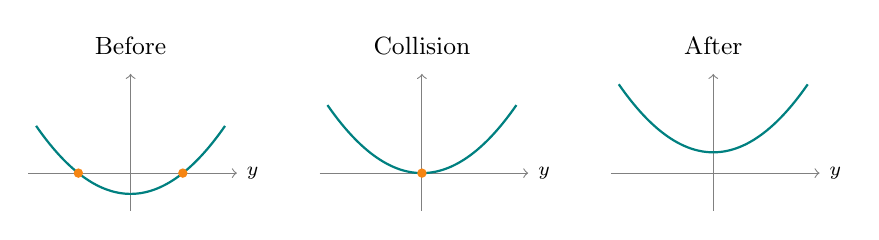
\begin{tikzpicture}[x=1cm,y=1.2cm]
 \foreach \shift/\ss/\title in {0/-0.22/Before,3.7/0/Collision,7.4/0.22/After}{
  \begin{scope}[xshift=\shift cm]
   \draw[->,gray] (-1.3,0)--(1.35,0) node[right,black] {\(\scriptstyle y\)};
   \draw[->,gray] (0,-0.4)--(0,1.05);
   \draw[thick,teal,domain=-1.2:1.2,samples=70]
    plot (\x,{0.5*\x*\x+\ss});
   \node at (0,1.35) {\small\title};
  \end{scope}
 }
 \fill[BurntOrange] (-0.6633,0) circle (1.7pt);
 \fill[BurntOrange] (0.6633,0) circle (1.7pt);
 \fill[BurntOrange] (3.7,0) circle (1.7pt);
\end{tikzpicture}
\caption{The universal quadratic model \(h/a=y^2/2+s\), with increasing
imaginary time from left to right. It illustrates the local analytic
law and is not a plot of theta data.}
\label{fig:fold}
\end{figure}

\subsection{A regular squared gap and the surrounding factor}
The symmetric functions constructed above define a monic quadratic
factor. Local analytic factorization gives
\begin{equation}\label{eq:local-factor}
 h(\tau,x)=(x-z_-(\tau))(x-z_+(\tau))U(\tau,x),
\end{equation}
where \(U\) is analytic and nonzero near the event. One may obtain the
quadratic's coefficients from the contour integrals of
\(x^k h_x/h\) around the fixed disk, which are analytic in \(\tau\);
division removes precisely the two enclosed roots. The quotient is a
holomorphic unit, including at \(s=0\). This is the same local
factorization used in the earlier heat-multiplicity analysis
\cite{HeatMultiplicity}. No product over all zeros is required.

For \(s<0\), write \(r_\pm=z_\pm\), \(\delta=r_+-r_->0\), and
\(q=\delta^2\). Let \(g=U_x/U\).

\begin{proposition}[Pair motion and squared gap]\label{prop:gap}
On the real-pair side,
\begin{align}
 r_\pm'&=-\frac{2}{r_\pm-r_\mp}-2g(\tau,r_\pm),\label{eq:pair-motion}\\
 \delta'&=-\frac4\delta-2\bigl(g(\tau,r_+)-g(\tau,r_-)\bigr),\label{eq:delta}\\
 q'&=-8-4q\int_0^1g_x(\tau,r_-+t\delta)\dd t.\label{eq:q-exact}
\end{align}
The squared gap extends analytically through the event and
\begin{equation}\label{eq:q-expansion}
 q(\tau_*+s)=-8s+16B_*s^2+O(s^3),\qquad
 B_*=\frac{c}{6a}-\frac{b^2}{9a^2}.
\end{equation}
The midpoint has velocity \(-2b/(3a)\) at the event.
\end{proposition}
\begin{proof}
At a simple zero \(r\), implicit differentiation gives
\(r'=-h_{xx}/h_x\). Differentiating \eqref{eq:local-factor} twice
at \(r_\pm\) yields
\[
 \frac{h_{xx}}{h_x}(\tau,r_\pm)
 =\frac{2}{r_\pm-r_\mp}+2g(\tau,r_\pm).
\]
Subtracting proves \eqref{eq:delta}; multiplying by \(2\delta\) and
using the fundamental theorem of calculus gives \eqref{eq:q-exact}.
Analyticity of the symmetric functions makes \(q\) analytic.
At \(s=0\),
\[
 U(\tau_*,x_*+y)=\frac a2+\frac b6y+\frac c{24}y^2+O(y^3),
\]
so \(g_*=b/(3a)\) and \(g_{x,*}=B_*\).
The integral in \eqref{eq:q-exact} tends to \(B_*\); its symmetric
expansion is \(B_*+O(s)\), since the midpoint is \(O(s)\) from \(x_*\)
and \(\delta^2=O(s)\). Thus \(q'(0)=-8\) and \(q''(0)=32B_*\),
proving \eqref{eq:q-expansion}. Adding the two root equations cancels
their singular terms and gives the midpoint velocity \(-2g_*\).
\end{proof}

The critical point and root midpoint generally have different velocities:
\(-b/a\) and \(-2b/(3a)\). Individual zero velocities diverge as
\(|s|^{-1/2}\), whereas both collective coordinates remain regular.
The term \(-8\) in \eqref{eq:q-exact} is the universal terminal closing
rate of a separated collision. The regular factor affects drift
and subsequent terms; this is not a uniform estimate on its size.

Rodgers and Tao's zero dynamics and gap law have the corresponding
decomposition with the opposite Newman-time sign
\cite[Section~4, Theorem~4.16 and Lemma~4.18(i)]{RodgersTao2020}.
Their printed theorem uses principal-value sums on the paper's
contradiction interval \(\Lambda<t\leq0\). We do not extend that theorem
to a different interval or to arbitrary nonreal zero configurations.
The local derivation above requires only the analytic factor \(U\).


\subsection{Amplitude, drift and relative curvature}
The coefficients in \eqref{eq:critical-place}--\eqref{eq:critical-value}
separate naturally into the amplitude \(a\) and two quantities unchanged
by a nonzero constant rescaling of the field:
\begin{equation}\label{eq:beta-gamma}
 \beta=\frac ba,\qquad \gamma=\frac ca-\frac{b^2}{a^2}.
\end{equation}
At the event, \(x_c'=-\beta\), \(v'=a\), and \(v''=a\gamma\).
At the reflected event, \(a,\gamma\) are unchanged and \(\beta\)
changes sign. The critical curve is the curve of stationary points
\(h_x=0\), not a curve of zeros of \(h\).

\begin{proposition}[Curvature transport and an event coordinate]
\label{prop:curvature-transport}
Along a regular critical curve, set
\(A(\tau)=h_{xx}(\tau,x_c(\tau))\ne0\) and \(r_c=-v/A\).
Then
\begin{align}
 A'&=h_{xxxx}-\frac{h_{xxx}^2}{h_{xx}},\qquad
 \frac{d}{d\tau}\log|A|
 =\frac{h_{xxxx}}{h_{xx}}-\frac{h_{xxx}^2}{h_{xx}^2},
 \label{eq:A-transport}\\
 r_c'&=-1-r_c\frac{A'}{A}.\label{eq:rc-transport}
\end{align}
In particular \(r_c(\tau_*+s)=-s+\tfrac12\gamma s^2+O(s^3)\)
and \(r_c\sim q/8\sim\tau_*-\tau\) on the real-pair side.
\end{proposition}
\begin{proof}
Differentiate \(A\) along the curve and use
\(x_c'=-h_{xxx}/h_{xx}\) and \(h_\tau=h_{xx}\).
The quotient rule and \(v'=A\) give \eqref{eq:rc-transport}.
Finally \(v=as+a\gamma s^2/2+O(s^3)\) and
\(A=a+a\gamma s+O(s^2)\), proving the expansion and, with
\eqref{eq:q-expansion}, the comparison.
\end{proof}

Thus \(\gamma\) is the relative rate of change of the extremum's
curvature. The regular event coordinates describe the same crossing;
they do not impose independent restrictions on it.

At the collision slice use the local factor \(U\) in
\eqref{eq:local-factor}, and write
\begin{equation}\label{eq:ell-kappa}
 \ell=\frac{U_x}{U}(\tau_*,x_*),\qquad
 \kappa=\partial_x\!\left(\frac{U_x}{U}\right)(\tau_*,x_*).
\end{equation}
The derivatives of \(h=(x-x_*)^2U\) give
\(U_*=a/2\), \(U_{x,*}=b/6\), \(U_{xx,*}=c/12\). Therefore
\begin{equation}\label{eq:coefficient-dictionary}
 \boxed{\ \beta=3\ell,\qquad c/a=6(\kappa+\ell^2),\qquad
 \gamma=6\kappa-3\ell^2,\qquad B_*=\kappa.\ }
\end{equation}
The same exterior curvature controls the second-order gap correction
and, together with the drift, the second-order critical value.

\subsection{A conditional real-zero benchmark}
\begin{proposition}[Exterior inverse-square curvature]
\label{prop:LP-coefficients}
Suppose additionally that the collision slice belongs to the real
Laguerre--P\'olya class. If its product has Gaussian factor
\(\ee^{-\alpha z^2}\), \(\alpha\ge0\), and \(\{\rho_j\}\)
are its remaining zeros, with multiplicities, after the two at \(x_*\)
are removed, then
\begin{equation}\label{eq:LP-kappa}
 \kappa=-2\alpha-\sum_j\frac{1}{(x_*-\rho_j)^2}.
\end{equation}
For an even slice with \(x_*\ne0\),
\begin{equation}\label{eq:LP-gamma}
 \kappa\le-\frac{1}{2x_*^2},\qquad
 \gamma\le-\frac{3}{x_*^2}-\frac{\beta^2}{3}<0.
\end{equation}
\end{proposition}
\begin{proof}
The defining canonical product is
\(Cz^m\ee^{-\alpha z^2+d z}
\prod_j(1-z/\rho_j)\ee^{z/\rho_j}\), with real parameters and zeros,
and \(\sum_{\rho_j\ne0}|\rho_j|^{-2}<\infty\)
\cite[Definition~1.1]{Csordas2014PositiveKernels}.
After removing the pair at \(x_*\), take the second logarithmic
derivative. The linear exponential and regularizing linear terms
disappear, giving \eqref{eq:LP-kappa}. The sum converges absolutely
locally off the remaining zeros; only finitely many are nearby and
the distant terms are bounded by a constant times \(|\rho_j|^{-2}\).
Evenness supplies a double zero at \(-x_*\), whose contribution is
\(-2/(2x_*)^2\). All other terms are nonpositive. Equation
\eqref{eq:coefficient-dictionary} proves \eqref{eq:LP-gamma}.
\end{proof}

This is a conditional benchmark for an all-real slice, not an
unconditional theta estimate. The weaker assertion \(\gamma\le0\)
also follows from the derivative Laguerre inequality \(b^2-ac\ge0\).
For \(a>0\), \eqref{eq:LP-gamma} says that a rising minimum
decelerates; its transverse crossing remains possible. The polynomial
\((x^2-r^2)^2\) has \(\beta=3/r\), \(\gamma=-6/r^2\) at \(r\)
and attains the displayed reflected-pair bound. This is a check of
the sharp constant, not a canonical-source example.

The sign changes when exterior zeros need not be real. An exterior
conjugate pair \(d\pm\ii\eta\) contributes
\begin{equation}\label{eq:complex-exterior-curvature}
 -\frac{2((x_*-d)^2-\eta^2)}{((x_*-d)^2+\eta^2)^2}
\end{equation}
to the logarithmic curvature, which may have either sign. A collision
at an all-real boundary and a later collision among a nonreal
background therefore require different estimates. The local theory
neither assumes nor proves that the global Newman threshold is
attained at one finite collision.

Finally, a bounded exterior correction by itself cannot oppose the
terminal closing rate. If the integral in \eqref{eq:q-exact} has
absolute value at most \(C>0\), then
\(q'\le-8+4Cq\le-4\) whenever \(0<q\le1/C\).
If this bound and cluster isolation persist, the pair closes in
at most \(q(\tau_0)/4\) further imaginary time. Preventing entry
into that regime requires information in addition to boundedness
of the regular factor.

\section{Coefficients from the complete theta source}\label{sec:coefficients}

The preceding identities isolate what must be estimated. We now
express the coefficients using the actual source and its primitive,
retaining all signed terms and endpoint contributions.

\subsection{Signed source moments}
At \(\lambda_* =\lambda_0-\tau_*\), define
\begin{equation}\label{eq:coefficient-moments}
 C_j=\int_0^\infty u^j F_{\lambda_*}(u)\cos(x_*u)\dd u,
 \qquad
 S_j=\int_0^\infty u^j F_{\lambda_*}(u)\sin(x_*u)\dd u.
\end{equation}
The complete bounds of Section~\ref{sec:source} justify
differentiation under each integral. At a collision they give
\begin{align}
 C_0&=S_1=0,\qquad a=-C_2,\quad b=S_3,\quad c=C_4,
 \label{eq:moment-jets}\\
 \beta&=-\frac{S_3}{C_2},\qquad
 \gamma=-\frac{C_2C_4+S_3^2}{C_2^2}.
 \label{eq:moment-ratios}
\end{align}
These formulas hold for the complete arithmetic source. Positivity
of \(F_{\lambda_*}\) does not make the signed cosine moments a
positive moment matrix. Separate absolute bounds on \(C_2,S_3,C_4\)
do not bound their ratios without a lower bound on \(|C_2|\).
A coupled estimate or an independently controlled exterior factor
would provide additional information; the formulas alone do not.

\subsection{The half-line primitive and its endpoint}
Use the restriction to \(u\ge0\) of the function \(A\) in
Section~\ref{sec:source}, now denoted by
\begin{equation}\label{eq:p-primitive}
 p(u)=\ee^u\sum_{n\ge1}\ee^{-\pi n^2\ee^{4u}},\qquad
 p''-p=8\Phi,\qquad p'(0)=-\tfrac12.
\end{equation}
The differential identity follows by termwise differentiation;
differentiating \(A(-u)-A(u)=\sinh u\) at zero proves the endpoint.
The same double-exponential majorants as before, with the corresponding
lower-degree polynomials, justify all integrations below. Set
\begin{equation}\label{eq:J-primitive}
 J_\lambda(x)=\int_0^\infty p(u)\ee^{\lambda u^2}\cos(xu)\dd u.
\end{equation}
Here \(J_\lambda\) is distinct from the absolute majorants
\(J_{r,d}\) in \eqref{eq:J}.

\begin{proposition}[Exact primitive transfer]\label{prop:primitive-transfer}
For every finite real \(\lambda,x\),
\begin{equation}\label{eq:primitive-transfer}
 8H_\lambda(x)=\tfrac12+(2\lambda-1-x^2)J_\lambda(x)
       +4\lambda xJ_\lambda'(x)-4\lambda^2J_\lambda''(x).
\end{equation}
For \(n\ge2\), with primes denoting spatial derivatives,
\begin{align}
 8H_\lambda^{(n)}={}&-4\lambda^2J_\lambda^{(n+2)}
 +4\lambda xJ_\lambda^{(n+1)}
 +(2\lambda-1-x^2+4\lambda n)J_\lambda^{(n)}\notag\\
 &-2nxJ_\lambda^{(n-1)}-n(n-1)J_\lambda^{(n-2)}.
 \label{eq:primitive-jets}
\end{align}
In particular \(a,b,c\) require primitive derivatives only through
orders four, five and six respectively.
\end{proposition}
\begin{proof}
For the smooth decaying tests used here, two integrations by parts give
\begin{equation}\label{eq:primitive-IBP}
 8\int_0^\infty\Phi f\dd u
 =\tfrac12 f(0)+p(0)f'(0)
       +\int_0^\infty p(f''-f)\dd u.
\end{equation}
Indeed the endpoint term is
\([p'f-pf']_0^\infty=-p'(0)f(0)+p(0)f'(0)\).
For \(f(u)=\ee^{\lambda u^2}\cos(xu)\), \(f(0)=1\), \(f'(0)=0\),
and
\[
 f''-f=\ee^{\lambda u^2}
 \bigl((2\lambda-1-x^2+4\lambda^2u^2)\cos(xu)
                   -4\lambda xu\sin(xu)\bigr).
\]
Replacing the last two integrals by \(-J_\lambda''\) and
\(-J_\lambda'\) proves \eqref{eq:primitive-transfer}.
Leibniz' rule for the quadratic and linear coefficients proves
\eqref{eq:primitive-jets}. All differentiations and vanishing
boundary terms are uniform on compact parameter sets by the paid
primitive tails.
\end{proof}

At \(\lambda=0\) this reduces to
\(8H_0=\tfrac12-(1+x^2)J_0\). A hypothetical collision on that
slice would consequently satisfy
\[
 J_0(x_*)=\frac{1}{2(1+x_*^2)},\qquad
 J_0'(x_*)=-\frac{x_*}{(1+x_*^2)^2}.
\]
The higher derivatives still contain the coefficient information.
The constant \(1/2\) in \eqref{eq:primitive-transfer} cannot be
dropped. Nor does positivity of \(p\) assert positivity of its
oscillatory transform or of the displayed signed combinations.

This half-line primitive is different from the smooth full-line
Green field \(G_\lambda\) in \eqref{eq:G-transform}.
In general \(G_\lambda\ne\ee^{\lambda u^2}G_0\); the latter is
not even integrable when \(\lambda>0\), by \eqref{eq:G-tail}.
The primitive identity is an exact alternative source representation,
with no estimating advantage claimed merely from the transfer.

\subsection{Recovering the exterior coefficients on a contour}
The local factor also has an interface that avoids division by the
vanishing value \(h(\tau_*,x_*)\). Let \(\Gamma\) be a positively
oriented simple contour bounding a disk that contains exactly the
two-root cluster, with multiplicity, and no boundary zero. Factor
\(H=P U\) there, with \(P\) the monic quadratic and \(U\) nonzero.
For \(z\) inside the contour define
\begin{equation}\label{eq:contour-A}
 \mathcal A_H(z)=\frac{1}{2\pi\ii}\oint_\Gamma
       \frac{H'(\zeta)/H(\zeta)}{\zeta-z}\dd\zeta.
\end{equation}
Then
\begin{equation}\label{eq:contour-exterior}
 \mathcal A_H(z)=\frac{U'(z)}{U(z)},\qquad
 \ell=\mathcal A_H(x_*),\quad \kappa=\mathcal A_H'(x_*).
\end{equation}
To prove this, subtract \(P'/P\) from \(H'/H\) and apply
Cauchy's formula to \(U'/U\). For \(z\) off the roots, each
term \(1/(\zeta-r)\) in \(P'/P\) contributes two opposite
residues to \eqref{eq:contour-A}, at \(r\) and \(z\).
Its integral is zero. Analytic continuation gives the formula at
the roots as well. Differentiating under the contour integral
gives the denominator \((\zeta-z)^2\) for \(\kappa\).
This is the existing local exterior-force interface, reused here
for the critical coefficients \cite{RTLocalTransfer}.

For clarity, its error payment can be stated explicitly. Suppose
on \(\Gamma\), \(|H|\ge m>0\),
\(|\widehat H-H|\le e_0<m\), \(|\widehat H'-H'|\le e_1\),
and \(|H'|\le M_1\). Then
\[
 \left|\frac{\widehat H'}{\widehat H}-\frac{H'}H\right|
 \le \frac{e_1}{m-e_0}+\frac{M_1e_0}{m(m-e_0)}=:D.
\]
If the length of \(\Gamma\) is \(L_\Gamma\) and its distance
from \(z\) is at least \(d>0\), the errors in \(\mathcal A_H(z)\)
and \(\mathcal A_H'(z)\) are at most
\(L_\Gamma D/(2\pi d)\) and \(L_\Gamma D/(2\pi d^2)\).
These follow directly by integrating the ratio error. The method
needs a boundary margin, a paid cluster count and complete source
errors; it does not need an internal pair-gap lower bound.
Its advantage, if any, is a quantitative comparison on a stated
region, not a consequence of introducing the contour.

\section{Mass and energy of the disappearing sign region}\label{sec:lobe}

The local geometry determines quantitative scales without evaluating
the theta function. Let \(\epsilon=\tau_*-\tau>0\) and
\(I_\tau=(r_-(\tau),r_+(\tau))\), on the real-pair side of the
collision. The amplitude has the sign opposite to \(a\) in this interval.

\begin{theorem}[Shrinking-lobe asymptotics]\label{thm:lobe}
As \(\epsilon\downarrow0\),
\begin{align}
 \int_{I_\tau}|h|\,\dd x
 &\sim\frac{4\sqrt2}{3}|a|\epsilon^{3/2},\label{eq:lobe-L1}\\
 M_{\mathrm{loc}}(\tau):=\int_{I_\tau}h^2\dd x
 &\sim\frac{16\sqrt2}{15}a^2\epsilon^{5/2},\label{eq:lobe-M}\\
 T_{\mathrm{loc}}(\tau):=\int_{I_\tau}h_x^2\dd x
 &\sim\frac{4\sqrt2}{3}a^2\epsilon^{3/2}.\label{eq:lobe-T}
\end{align}
Consequently
\begin{equation}\label{eq:lobe-Rayleigh}
 \frac{T_{\mathrm{loc}}}{M_{\mathrm{loc}}}
 \sim\frac{5}{4\epsilon}.
\end{equation}
\end{theorem}
\begin{proof}
Use \(x=x_*+\sqrt{2\epsilon}\,t\). By
\eqref{eq:heat-four-jet}, uniformly for \(t\) in a fixed bounded interval,
\[
 \frac{h(\tau_*-\epsilon,x_*+\sqrt{2\epsilon}\,t)}{\epsilon}
 =a(t^2-1)+O(\epsilon^{1/2}),
\]
and
\[
 \frac{h_x(\tau_*-\epsilon,x_*+\sqrt{2\epsilon}\,t)}
      {\sqrt{2\epsilon}}
 =at+O(\epsilon^{1/2}).
\]
The scaled endpoints tend to \(-1\) and \(1\), by
Theorem~\ref{thm:splitting}. The expansions give uniform bounds on
a common interval containing them, so dominated convergence applies
also to the varying integration intervals. The three limiting
integrals are
\[
 \int_{-1}^1(1-t^2)\dd t=\frac43,\qquad
 \int_{-1}^1(1-t^2)^2\dd t=\frac{16}{15},\qquad
 \int_{-1}^1t^2\dd t=\frac23.
\]
Restoring the factors \(\sqrt{2\epsilon}\), \(\epsilon\) and
\(\sqrt{2\epsilon}\) proves \eqref{eq:lobe-L1}--\eqref{eq:lobe-T}.
Their quotient gives \eqref{eq:lobe-Rayleigh}.
\end{proof}

The angular-integrated field mass and radial kinetic form in this
interval are \((2/\pi)M_{\mathrm{loc}}\) and
\((2/\pi)T_{\mathrm{loc}}\). Their ratio is unchanged. Both contributions
vanish at the collision. The divergence in \eqref{eq:lobe-Rayleigh}
is produced by normalizing a region whose mass vanishes faster than
its kinetic form; it is compatible with all the global regularity and
dissipation laws in Proposition~\ref{prop:global-energy}.

This quotient is a local Dirichlet quadratic form. The restriction of
\(h\) to \(I_\tau\), extended by zero, belongs to \(H^1(\R)\), since its
boundary values vanish. Its derivative generally jumps at the simple
endpoints, so the extension need not belong to \(H^2(\R)=\Dom B\).
Thus \eqref{eq:lobe-Rayleigh} is not being promoted to an operator
expectation of an arbitrarily cut-off state in the full domain.
Nor is a physical conditioning operation introduced by the
normalization.

At the event itself, \eqref{eq:heat-four-jet} gives
\begin{equation}\label{eq:local-density-scales}
 h(\tau_*,x_*+y)^2=\frac{a^2}{4}y^4+O(y^5),\qquad
 h(\tau_*+s,x_*)^2=a^2s^2+O(s^3).
\end{equation}
The local intensity therefore develops a quartic spatial zero and
refills quadratically in time, consistently with
\eqref{eq:density-event}. In the real amplitude, two sign transitions
disappear when the intervening pocket closes.

It is useful to compare three different notions of size near the same
event. The full norm and field energy are finite; the local lobe mass
and energy vanish; and the normalized local quotient diverges. Singular
zero-configuration quantities provide another example:
\[
 -\log\delta\sim-\tfrac12\log(8\epsilon),\qquad
 \delta^{-2}\sim(8\epsilon)^{-1}.
\]
These are functions of the zero coordinates, not the field expectation
\(\inner{\Psi}{K\Psi}\). The formal global zero Hamiltonians and
energies in \cite{RodgersTao2020} require their own truncation and
convergence analysis. Their singularity cannot be identified with a
failure of the smooth cylinder evolution.


\subsection{Exact balances on a moving sign region}
The asymptotic constants fit exact identities valid before the
collision. Write \(L_{\mathrm{loc}}=\int_{I_\tau}|h|\dd x\).
\begin{proposition}[Moving-boundary dissipation]\label{prop:lobe-balance}
As long as the endpoints are simple zeros bounding one sign region,
\begin{align}
 L_{\mathrm{loc}}'&=-|h_x(\tau,r_-)|-|h_x(\tau,r_+)|,
 \label{eq:lobe-L-balance}\\
 M_{\mathrm{loc}}'&=-2T_{\mathrm{loc}},
 \qquad \frac{T_{\mathrm{loc}}}{M_{\mathrm{loc}}}
       =-\tfrac12(\log M_{\mathrm{loc}})',
 \label{eq:lobe-M-balance}\\
 T_{\mathrm{loc}}'&=[h_xh_{xx}]_{r_-}^{r_+}
             -2\int_{I_\tau}h_{xx}^2\dd x.
 \label{eq:lobe-T-balance}
\end{align}
\end{proposition}
\begin{proof}
The boundary values of \(|h|\) and \(h^2\) vanish. If \(\sigma\)
is the sign of \(h\) in the region, differentiating its area gives
\(\sigma\int h_{xx}=\sigma[h_x]_{r_-}^{r_+}\), equal to
the negative sum in \eqref{eq:lobe-L-balance}.
Integration by parts gives
\(M_{\mathrm{loc}}'=2\int hh_{xx}=-2\int h_x^2\).
For the kinetic form, retain the endpoint velocities:
\[
 T_{\mathrm{loc}}'=h_x(r_+)^2r_+'-h_x(r_-)^2r_-'
                       +2\int_{I_\tau}h_xh_{xxx}\dd x.
\]
Using \(r_\pm'=-h_{xx}/h_x\) and integrating the last term
by parts leaves exactly \eqref{eq:lobe-T-balance}.
\end{proof}

The boundary term in \eqref{eq:lobe-T-balance} is essential: the
whole-line kinetic dissipation law does not apply unchanged to a
moving region. Equations \eqref{eq:lobe-M-balance} and
\eqref{eq:lobe-M} are consistent with the coefficient \(5/4\)
in \eqref{eq:lobe-Rayleigh}; that coefficient was proved from the
two integrals, without differentiating an uncontrolled asymptotic
remainder. In terms of the actual gap,
\begin{equation}\label{eq:lobe-gap-scales}
 L_{\mathrm{loc}}\sim\frac{|a|\delta^3}{12},\quad
 M_{\mathrm{loc}}\sim\frac{a^2\delta^5}{120},\quad
 T_{\mathrm{loc}}\sim\frac{a^2\delta^3}{12},\quad
 \delta^2\frac{T_{\mathrm{loc}}}{M_{\mathrm{loc}}}\longrightarrow10.
\end{equation}
These follow from \(\delta^2\sim8\epsilon\). Here
\(\epsilon=\tau_*-\tau=\lambda-\lambda_*\) is remaining time
to the event, not an error term or a source perturbation.

\section{Interference balances and source response}\label{sec:interference}

The local normal form describes what a collision does. The integral
representation describes what must balance for it to occur. We derive
two complementary descriptions, using momentum damping and spatial
heat averaging. Neither description, by itself, forbids the event.

\subsection{Positive momentum source, signed cosine observation}
At the collision, differentiation of \eqref{eq:F-H} gives
\begin{align}
 \int_0^\infty F_{\lambda_*}(u)\cos(x_*u)\dd u&=0,\label{eq:cos-balance}\\
 \int_0^\infty uF_{\lambda_*}(u)\sin(x_*u)\dd u&=0,\label{eq:sin-balance}\\
 \int_0^\infty u^2F_{\lambda_*}(u)\cos(x_*u)\dd u&=-a\ne0,
 \label{eq:curvature-balance}
\end{align}
where \(\lambda_*=\lambda_0-\tau_*\).
Thus a strictly positive source can produce a double node through two
signed observation balances. The second moment in
\eqref{eq:curvature-balance} measures the transverse crossing.

Fix the observation point \(x_*\), and put
\[
 c_\pm(u)=\max\{\pm\cos(x_*u),0\},\quad
 A_\pm(\tau)=\int_0^\infty F_{\lambda_0-\tau}(u)c_\pm(u)\dd u,
\]
\[
 B_\pm(\tau)=
 \frac{\int_0^\infty u^2F_{\lambda_0-\tau}(u)c_\pm(u)\dd u}
      {A_\pm(\tau)}.
\]
Since \(x_*\ne0\), both cosine signs occupy open intervals and
\(A_\pm>0\). Dominated differentiation in time yields
\begin{equation}\label{eq:sector-damping}
 A_\pm'=-A_\pm B_\pm,\qquad
 \frac{\dd}{\dd\tau}\log\frac{A_+}{A_-}=-(B_+-B_-).
\end{equation}
At the event \(A_+=A_-=:A\), and
\begin{equation}\label{eq:sector-curvature}
 a=-A(B_+-B_-).
\end{equation}
If \(a>0\), the negative cosine sector has the larger mean \(u^2\)
and therefore damps faster. The observed amplitude rises through zero.
If \(a<0\), the positive sector damps faster and the crossing is downward.
Equation~\eqref{eq:sin-balance} is the additional stationarity constraint;
the sector-mass equality alone is only a zero condition.

These means use the \emph{linear} source, not the squared-amplitude
measure \eqref{eq:spectral-measure}. The corners of \(c_\pm\) cause no
difficulty for the time derivatives above: the observation point is
fixed and the source moments dominate the integrands. No spatial
differentiation through moving sector boundaries is being used.

\subsection{A spatial heat-average balance}
Choose \(0<\Delta\leq\tau_*\), and define
\[
 k_\Delta(y)=(4\pi\Delta)^{-1/2}\ee^{-y^2/(4\Delta)},\qquad
 f(y)=h(\tau_*-\Delta,y).
\]
The heat multiplier gives \(h(\tau_*,x)=k_\Delta*f(x)\).
This identity first holds in \(L^2\); the integral and all its displayed
derivatives are continuous by Cauchy--Schwarz against Gaussian
derivatives, so it also holds pointwise. Define a signed measure
\[
 \dd\mu(y)=k_\Delta(x_*-y)f(y)\dd y.
\]
Its absolute moments of every fixed order are finite. Differentiating
the Gaussian proves
\begin{equation}\label{eq:gaussian-moments}
 \int\dd\mu=0,\qquad
 \int(y-x_*)\dd\mu=0,\qquad
 \int(y-x_*)^2\dd\mu=4\Delta^2a.
\end{equation}
Indeed, \(\partial_x k_\Delta(x-y)=(y-x)k_\Delta/(2\Delta)\);
the second derivative is
\(\bigl((y-x)^2/(4\Delta^2)-1/(2\Delta)\bigr)k_\Delta\).
The zeroth moment vanishes, removing the last term.

Let \(\mu=\mu_+-\mu_-\) be the positive and negative parts.
Since \(a\ne0\), neither is zero. The first two identities imply
\[
 \mu_+(\R)=\mu_-(\R)=:M>0,\qquad
 \frac1M\int y\dd\mu_+=\frac1M\int y\dd\mu_-=:m.
\]
Writing \(\sigma_\pm^2=M^{-1}\int(y-m)^2\dd\mu_\pm\), the last
identity becomes
\begin{equation}\label{eq:variance-balance}
 a=\frac{M}{4\Delta^2}(\sigma_+^2-\sigma_-^2).
\end{equation}
Thus the earlier positive and negative amplitudes, after Gaussian
weighting about the future event, have equal masses and centroids.
Their variance difference supplies the nonzero crossing curvature.
This is an exact conditional description of a collision, valid at
any such earlier time; it is not an estimate that excludes one.

\subsection{Smooth displacement under source perturbation}
The divergent velocity of an individual zero does not imply singular
dependence of the \emph{joint event} on source parameters.
Let \(q(u)\) be a real, even, bounded smooth function whose derivatives
have polynomial growth, and perturb the supplied source to
\[
 F_{\lambda,\eta}(u)=\ee^{\lambda u^2+\eta q(u)}\Phi(u).
\]
The moment bounds and Schwartz properties persist on compact
parameter sets. The resulting field \(h_\eta\) is analytic in
\((\tau,x,\eta)\), with
\[
 r(\tau,x):=\left.\partial_\eta h_\eta(\tau,x)\right|_{\eta=0}
 =\int_0^\infty F_{\lambda_0-\tau}(u)q(u)\cos(xu)\dd u.
\]

\begin{proposition}[Event response]\label{prop:response}
A collision of \(h_0\) continues uniquely as an analytic local
event \((\tau_*(\eta),x_*(\eta))\). At \(\eta=0\),
\begin{equation}\label{eq:event-response}
 \tau_*'=-\frac{r}{a},\qquad
 x_*'=\frac{br}{a^2}-\frac{r_x}{a},
\end{equation}
where the right-hand side is evaluated at the unperturbed event.
\end{proposition}
\begin{proof}
Apply the analytic implicit-function theorem to
\((h_\eta,\partial_xh_\eta)=0\). Its Jacobian in \((\tau,x)\) is
\[
 \begin{pmatrix}h_\tau&h_x\\h_{x\tau}&h_{xx}\end{pmatrix}_{*}
 =\begin{pmatrix}a&0\\b&a\end{pmatrix},
\]
with determinant \(a^2\ne0\). Differentiation of the two event equations
gives \(a\tau_*'+r=0\) and \(b\tau_*'+ax_*'+r_x=0\), proving
\eqref{eq:event-response}.
\end{proof}

This is the source-response calculation of
\cite{SourceResponse} in the present time convention.
It is local at a nondegenerate event, not uniform as \(a\to0\).
A general tilt changes the canonical theta arithmetic. The proposition
therefore explains event stability and sensitivity without furnishing
a permitted deformation of the canonical source or proving that its
event exists.

\section{Higher multiplicity and singular observation coordinates}
\label{sec:multiplicity}

\subsection{The finite heat-polynomial normal form}
Suppose a real event has exact spatial order \(m\geq2\):
\[
 \partial_x^jh(\tau_*,x_*)=0\quad(0\leq j<m),\qquad
 a_m=\partial_x^mh(\tau_*,x_*)\ne0.
\]
For fixed \(m\), define
\begin{equation}\label{eq:heat-poly}
 p_m(S,Y)=
 \sum_{j=0}^{\lfloor m/2\rfloor}
 \frac{m!}{j!(m-2j)!}S^jY^{m-2j}.
\end{equation}

\begin{theorem}[Finite-multiplicity heat geometry]\label{thm:higher}
Uniformly for \((S,Y)\) in compact sets,
\begin{equation}\label{eq:higher-rescale}
 h(\tau_*+\epsilon^2S,x_*+\epsilon Y)
 =\frac{a_m}{m!}\epsilon^m p_m(S,Y)+O(\epsilon^{m+1}).
\end{equation}
In a sufficiently small fixed complex neighborhood of \(x_*\), the
cluster consists of \(m\) simple real zeros immediately before the event.
Immediately after it, there are no real zeros if \(m\) is even, and
exactly one simple real zero if \(m\) is odd. The remaining zeros form
nonreal conjugate pairs; the total complex multiplicity stays \(m\).
\end{theorem}
\begin{proof}
The coefficient of \(s^jy^k\) in the local Taylor series is
\(\partial_x^{2j+k}h/(j!k!)\), by the heat equation. All terms of
parabolic weight \(2j+k<m\) vanish, and the weight-\(m\) terms give
\eqref{eq:heat-poly}. A finite Taylor remainder, as in
Section~\ref{sec:double}, proves \eqref{eq:higher-rescale}.

For completeness, the real-root property of \(q_m(Y)=p_m(-1,Y)\)
can be proved directly. The displayed coefficients give
\[
 q_0=1,\quad q_1=Y,\quad
 q_{m+1}=Yq_m-2m q_{m-1}.
\]
These monic polynomials have simple real interlacing zeros by induction.
At successive zeros of \(q_m\), the values of \(q_{m+1}=-2m q_{m-1}\)
alternate in sign, giving \(m-1\) intervening roots. At the largest
zero of \(q_m\), \(q_{m-1}>0\) and \(q_{m+1}<0\), whereas
\(q_{m+1}(Y)>0\) for large positive \(Y\), giving a further root.
At the smallest zero, the sign of \(q_{m-1}\) is \((-1)^{m-1}\);
the sign of \(q_{m+1}\) there is \((-1)^m\), opposite its sign at
large negative \(Y\). This supplies the last root. The degree is
\(m+1\), so all are simple and the interlacing is strict.
The induction begins with \(q_1=Y\) and \(q_2=Y^2-2\).
Parity shows that precisely the odd polynomials have a zero at zero.

Set \(s=-\epsilon^2\) before the event. Dividing the field by
\(\epsilon^m\) gives an analytic family in \((\epsilon,Y)\), including
\(\epsilon=0\), with limiting simple roots those of \(q_m\).
The implicit-function theorem continues every root as a real simple
root for small real positive \(\epsilon\).
After the event, \(s=\epsilon^2\), and
\[
 p_m(1,\ii Y)=\ii^m p_m(-1,Y).
\]
The nonzero limiting roots are therefore purely imaginary and stay
nonreal under a sufficiently small perturbation. If \(m\) is odd,
the limiting root at zero is simple and its unique continued branch
is real by conjugation symmetry. For even \(m\) there is no such root.
Finally, choose a fixed disk containing only the order-\(m\) zero at
the event. Its nonzero boundary and analytic convergence preserve the
total zero count \(m\). The branches just constructed exhaust it.
\end{proof}

This recovers the local forward-parabolic multiplicity pattern in
\cite{Angenent1991,HeatMultiplicity}. It asserts neither that all
canonical events have multiplicity two nor that one can choose the neighborhoods
or remainder constants uniformly in \(m\) or in height.

\subsection{What the generator detects at a node}
The complete operator intertwining gives, for each fixed \(j\),
\begin{equation}\label{eq:generator-jets}
 R_\chi K^j\Psi_\tau=(-1)^j\partial_x^{2j}h(\tau,\cdot).
\end{equation}
If \(m=2r\), the first nonzero pointwise value in this even-derivative
sequence is at \(j=r\). If \(m=2r+1\), the values for \(j\leq r\)
vanish, but the first spatial derivative of the \(j=r\) readout is
nonzero. These are justified pointwise statements for the prepared
smooth orbit. They do not assert bounded point evaluation on the
ambient \(L^2\) space. In particular, \(K\) and its powers are finite
on the source state even when lower-order readouts vanish.

\subsection{Logarithmic derivatives and their poles}
On an open region where \(h\ne0\), put \(w=h_x/h\).
Since \(h_\tau=h_{xx}\),
\[
 \partial_\tau\log h=\frac{h_{xx}}h=w_x+w^2,
\]
locally using any analytic logarithm. Differentiating in \(x\) gives
\begin{equation}\label{eq:burgers}
 w_\tau=w_{xx}+2ww_x.
\end{equation}
At a collision the local factorization gives
\[
 w(\tau_*,x_*+y)=\frac2y+\frac{b}{3a}+O(y),\qquad
 \frac{h_{xx}}h(\tau_*,x_*+y)=\frac2{y^2}+O(y^{-1}).
\]
These poles are created by division by the vanishing amplitude.
They are compatible with the regular field, regular generator
derivatives and regular energy identities already proved. Thus a
singularity in a logarithmic or root coordinate must be distinguished
from a singularity of the state.

All two-sided local statements concern the analytic source family
near an interior event. At the endpoint \(\tau=0\), a physical
semigroup orbit provides only the forward side. The entire source
formula still supplies a mathematical local extension, but it does
not make reverse evolution bounded on arbitrary ambient states.

\section{An explicit colliding source within the analytic class}
\label{sec:control}

The preceding local laws use heat evolution and strong source decay.
To identify what those premises can establish on their own, we give
an exact positive source satisfying them and having a collision.
This is a control for generic analytic or operator arguments, not a
replacement for the theta source.

For \(c_0>0\), define
\begin{equation}\label{eq:control-source}
 \Phi_{\mathrm c}(u)=c_0\ee^{-u^2/4}
 \left(\ee^{-u^4}+\frac12\ee^{-(u-4)^4}
                    +\frac12\ee^{-(u+4)^4}\right).
\end{equation}
It is real, even and strictly positive. If \(|u|\geq8\), then
\(|u\pm4|\geq|u|/2\), so the bracket is at most
\(2\ee^{-u^4/16}\). Every derivative is a finite sum of polynomial
factors times the same shifted exponentials and Gaussian.
Consequently \(F_{\lambda,\mathrm c}=\ee^{\lambda u^2}\Phi_{\mathrm c}\)
is Schwartz, has every fixed exponentially weighted absolute moment,
and lies in every fixed multiplier power domain, locally uniformly
in \(\lambda\). Its transform is jointly entire in \((\lambda,z)\).
The complete cylinder, first-shell preparation and readout of
Section~\ref{sec:operator} therefore apply unchanged.

\begin{proposition}[Exact collision]\label{prop:control}
At \(\lambda_*=1/4\), the cosine transform of
\eqref{eq:control-source} is
\begin{equation}\label{eq:control-transform}
 H_{\lambda_*,\mathrm c}(x)=c_0 Q(x)(1+\cos4x),\qquad
 Q(x)=\int_0^\infty\ee^{-u^4}\cos(xu)\dd u.
\end{equation}
It has a double zero at \(x_*=\pi/4\), with
\begin{align}
 a&=16c_0Q(x_*)>0,\label{eq:control-a}\\
 b&=48c_0Q'(x_*),\qquad
 c=96c_0Q''(x_*)-256c_0Q(x_*).\label{eq:control-bc}
\end{align}
For example, preparation at \(\lambda_0=1/2\) places this event
at the interior imaginary time \(\tau_*=1/4\).
\end{proposition}
\begin{proof}
At \(\lambda_*=1/4\), the Gaussian in \eqref{eq:control-source}
cancels. Translation by \(\pm4\) in the full Fourier integral
multiplies the transform of \(\ee^{-u^4}\) by
\(\ee^{\pm4\ii x}\). Evenness and the half-line normalization give
\eqref{eq:control-transform}.

We verify \(Q(x_*)>0\) without quadrature. Let
\(M_j=\int_0^\infty u^j\ee^{-u^4}\dd u\).
Integration of \((u\ee^{-u^4})'\) gives \(M_4=M_0/4\), and
Cauchy--Schwarz gives \(M_2\leq(M_0M_4)^{1/2}=M_0/2\).
The inequality \(\cos t\geq1-t^2/2\) implies
\[
 Q(x)\geq M_0-\frac{x^2}{2}M_2
       \geq M_0\left(1-\frac{x^2}{4}\right)>0
       \quad (|x|<2).
\]
Since \(x_*=\pi/4<2\), the factor \(Q\) is nonzero there.
The factor \(1+\cos4x\) has a double zero, second derivative \(16\),
third derivative \(0\) and fourth derivative \(-256\) there.
The product rule yields \eqref{eq:control-a}--\eqref{eq:control-bc}.
\end{proof}

The normalized coefficients also have an exact sign in this control:
\begin{equation}\label{eq:control-gamma}
 \beta=3Q'/Q,\qquad
 \gamma=6Q''/Q-9(Q'/Q)^2-16<-16
 \quad\text{at }x_*.
\end{equation}
To prove the strict inequality, the moment notation above gives
\(M_2\ge1/(3e)\) by integration over \([0,1]\), and
\(M_0\le1+1/e\), since \(u^4\ge u\) for \(u\ge1\).
Thus \(M_2/M_0\ge1/[3(e+1)]>1/12\). Applying
\(\cos t\ge1-t^2/2\) to \(-Q''\) yields
\[
 Q''(\pi/4)\le-M_2+\frac{\pi^2}{128}M_0<0,
\]
because \(\pi^2<10\) and \(10/128<1/12\).
Equation~\eqref{eq:control-bc} now proves \eqref{eq:control-gamma}.
This argument assumes no all-real-zero property of the control.
In particular, a negative critical-curvature coefficient alone
cannot exclude a collision.

The field and full operator energy are regular at this exact event,
while its roots and disappearing sign region obey all the laws above.
Thus positivity, evenness, super-Gaussian tails, entire continuation,
membership in all fixed power domains, and a nonnegative generator
do not jointly exclude collisions.

The premise this control fails is the \emph{exact canonical theta
arithmetic expansion} \eqref{eq:Phi}. Any canonical exclusion
must use further information from that source, beyond the analytic
properties shared by \eqref{eq:control-source}. This is a scoped
statement about the displayed premises. It does not rule out
source-specific estimates or every possible physical construction.

Other repository controls are documented in the operator assessment
\cite{OperatorAssessment}: atomic sources are not \(L^2\) source
states for this encoder, while broad positive-mixture and positive
coefficient examples require their own domain and continuation
checks. We do not claim a fresh family-wide audit of those examples.
For the control above, both the analytic bounds and the collision
are proved explicitly here.

\section{Exterior interactions and Rodgers--Tao renormalization}
\label{sec:RT}

\subsection{What the real-zero argument controls}
The factorization in Section~\ref{sec:double} removes the singular
mutual interaction of one pair. In the real Laguerre--P\'olya setting,
\(-\kappa\) is an exterior inverse-square sum, with the possible
Gaussian term in \eqref{eq:LP-kappa}. This connects the critical
coefficients to the interaction quantities in Rodgers and Tao's
proof \cite{RodgersTao2020}. Their theorem proves \(\Lambda\ge0\)
by contradiction from \(\Lambda<0\): real, simple zero dynamics
then exists on an interval reaching the zeta slice \(t=0\).
Here their parameter \(t\) is our Newman parameter \(\lambda\),
and has the opposite orientation to \(\tau\).

Their finite-block localization and renormalized energies control
deviations from classical spacing over growing blocks. The
definitions and estimates used here are those of corrected arXiv
version~5, Sections~4 and~7; HTML theorem numbers differ from the
journal/PDF numbering. We use the method and its scope, not an
unstated extension of its estimates to \(\Lambda>0\).

\subsection{Renormalization retains the collision pole}
For a positive actual separation \(g\) and reference separation
\(d>0\), the pair interaction is renormalized using
\begin{equation}\label{eq:RT-renorm}
 V(r)=r^{-2}-1+2(r-1),\qquad
 \widetilde E(g,d)=d^{-2}V(g/d).
\end{equation}
Since \(V(1)=V'(1)=0\) and \(V''(r)=6r^{-4}>0\), this is
nonnegative for \(r>0\). It subtracts the constant and linear
reference contribution, not the singular interaction. Indeed
\begin{equation}\label{eq:RT-pole}
 \widetilde E(g,d)=g^{-2}-3d^{-2}+2g d^{-3}
                =g^{-2}+O(1)\quad(g\downarrow0)
\end{equation}
at fixed \(d\). Ordered-pair sums count this term twice.
Neither \(\widetilde E\) nor \(-\kappa\) is the field energy
\(\inner\Psi{K\Psi}\) or the local quotient
\(T_{\mathrm{loc}}/M_{\mathrm{loc}}\).

The local deflation \(H=P U\) and the reference subtraction
\eqref{eq:RT-renorm} perform different jobs. The former gives a
regular local coefficient through a collision; the latter makes
a large real-zero interaction comparable with an equilibrium
configuration. An integrated estimate over growing blocks does
not by itself bound one prescribed exterior coefficient or
prevent an isolated finite-height event.

This leaves two distinct questions. One is whether the exact theta
source gives effective bounds on \(\ell,\kappa\) in a declared
cluster region, using \eqref{eq:moment-ratios} or
\eqref{eq:contour-exterior}. The other is whether a statistical
argument can be formulated when the zeros are not all real.
The latter requires retaining the transverse zero coordinates;
it is taken up in Section~\ref{sec:complex-statistics}. No extension of the Rodgers--Tao
relaxation theorem is presumed in making that definition.

\section{Bulk statistics and exceptional zeros}\label{sec:complex-statistics}

The transport identities describe a possible defect on the zeta slice.
Before localizing a statistical test around it, we identify what the
established bulk comparisons actually control. Their positivity and
asymptotic formulas concern different observables and different
quantifiers.

\subsection{Coordinates and the original comparison}
Write a nontrivial zeta zero as \(\rho=\sigma+\ii t\), where
\(0<\sigma<1\). To avoid confusing these coordinates with the
collision coefficients \(\beta,\gamma\), we use \(\sigma,t\)
throughout this section. Its corresponding zero of \(H_0\) is
\begin{equation}\label{eq:zeta-H-zero-map}
 z=2t+\ii(1-2\sigma).
\end{equation}
Thus a zero off the critical line is a \emph{nonreal} zero of
\(H_0\), not generally a purely imaginary one. A pure imaginary
zero of \(H_\lambda\), for real \(\lambda\), is impossible:
\(H_\lambda(\ii y)=\int_0^\infty F_\lambda(u)\cosh(yu)\dd u>0\).

Put \(L_T=(\log T)/(2\pi)\), \(B_T=TL_T\), and sum over all
zeros with \(0<t\le T\), counting multiplicity. The ordinate-only
Montgomery sum makes sense without RH:
\begin{equation}\label{eq:F-vertical}
 F_{\rm v}(\alpha,T)=\frac1{B_T}\sum_{\rho,\rho'}
 T^{\ii\alpha(t-t')}\frac4{4+(t-t')^2}.
\end{equation}
Its definition records vertical separation, but discards \(\sigma\).
Montgomery's original restricted-frequency asymptotic assumes RH
\cite[Theorem, equations (1)--(2)]{Montgomery1973}.
The full sine-kernel pair-correlation conjecture is stronger than
that theorem and is not a premise of the Rodgers--Tao proof.
Under \(\Lambda<0\), their dynamics forces almost all gaps at
\(\lambda=0\) to be asymptotic to their mean; their final
contradiction uses a positive proportion of smaller gaps
\cite[Section~9, equation (93)]{RodgersTao2020}. The proof there
uses the gap theorem of Conrey, Ghosh, Goldston, Gonek and
Heath-Brown, rather than assuming the full statistical conjecture.

\subsection{An unconditional complex-difference statistic}
Baluyot, Goldston, Suriajaya and Turnage-Butterbaugh instead retain
the complete difference of zeros. Define
\begin{equation}\label{eq:F-complex}
 F_{\rm c}(\alpha,T)=\frac1{B_T}\sum_{\rho,\rho'}
 T^{\alpha(\rho-\rho')}W(\rho-\rho'),\qquad
 W(u)=\frac4{4-u^2}.
\end{equation}
There is no pole in this sum since \(|\Re(\rho-\rho')|<1\).
Under RH, \(F_{\rm c}=F_{\rm v}\). Without RH they are different:
\(T^{\alpha(\rho-\rho')}\) includes the real factor
\(T^{\alpha(\sigma-\sigma')}\), and the kernel may be complex.

\begin{theorem}[Unconditional Montgomery theorem, imported]
\label{thm:BGST}
For the zeta zeros, \(F_{\rm c}\) is real, even in \(\alpha\),
and nonnegative. As \(T\to\infty\), uniformly for
\(0\le\alpha\le1\),
\begin{equation}\label{eq:BGST}
 F_{\rm c}(\alpha,T)
 =T^{-2\alpha}(\log T+O(1))+\alpha
                        +O((\log T)^{-1/2}).
\end{equation}
No RH assumption is required.
\end{theorem}
This is \cite[Theorem~1, (1.2)--(1.4)]{BGST2024}, in the
pinned arXiv version~1. Its arithmetic asymptotic is an imported
result. The following direct calculation explains why positivity
survives the presence of nonreal zeros.

\begin{proposition}[A positive integral for the finite sum]
\label{prop:complex-Gram}
For any finite multiset \(\mathcal Z\) in \(0<\Re\rho<1\)
invariant under \(\rho\mapsto1-\overline\rho\), and \(x>0\),
\begin{equation}\label{eq:complex-Gram}
 \sum_{\rho,\rho'\in\mathcal Z}x^{\rho-\rho'}W(\rho-\rho')
 =\int_\R\ee^{-2|v|}
 \left|\sum_{\rho\in\mathcal Z}
       \ee^{(\rho-1/2)(\log x+v)}\right|^2\dd v\ge0.
\end{equation}
\end{proposition}
\begin{proof}
For \(|\Re u|<2\), direct integration on the two half-lines gives
\(W(u)=\int_\R\ee^{-2|v|}\ee^{uv}\dd v\).
Relabel \(\rho'\) by \(1-\overline\rho'\). The summand becomes
\(x^{\rho+\overline\rho'-1}W(\rho+\overline\rho'-1)\).
Insert the integral and expand the absolute square. Finite
summation is legitimate; the largest real exponent in the
integrand has absolute value less than one, so the integral
converges. Swapping the two indices in the original expression
also proves invariance under \(x\mapsto1/x\).
\end{proof}

The published proof has an equivalent positive integral with
Cauchy kernels \cite[Lemma~3, (2.6)]{BGST2024}.
Thus the obstacle is not simply loss of positivity of the
statistic. Its summands, however, are not nonnegative pair
counts, and this positivity does not imply that each zero is
on the critical line. Analytic test functions at complex zero
coordinates also occur in the earlier higher-correlation theorem
of Rudnick and Sarnak \cite[Theorem~1.1]{RudnickSarnak1996};
its restricted Fourier support and entire smoothing must be
retained. It is not a theorem for arbitrary planar pair tests.

\subsection{What ordinate statistics can detect}
The functional equation pairs \(\sigma+\ii t\) with
\(1-\sigma+\ii t\). Consequently, even a statistic that discards
\(\sigma\) can detect the coincidence of their ordinates.
For each distinct ordinate \(t\), let \(m_t\) be the total
multiplicity of zeros on that horizontal line, and set
\begin{equation}\label{eq:horizontal-excess}
 N(T)=\sum_t m_t,\qquad D(T)=\sum_t m_t(m_t-1).
\end{equation}
The pair sum including all equal-ordinate terms is \(N(T)+D(T)\).
This is the horizontal-multiplicity observable studied by
Goldston, Lee, Schettler and Suriajaya
\cite[Sections~7--8]{GLSS2026}.

\begin{proposition}[Coincidence bounds]\label{prop:horizontal}
Let \(N_{\rm off}(T)\) count zeros off the critical line, with
multiplicity, and let \(N_{\rm sc}(T)\) count simple critical-line
zeros. Then
\begin{equation}\label{eq:horizontal-bounds}
 N_{\rm off}(T)\le D(T),\qquad
 N_{\rm sc}(T)\ge N(T)-D(T).
\end{equation}
In particular \(D(T)=o(N(T))\) implies that a proportion tending
to one of the zeros is simple and on the critical line.
\end{proposition}
\begin{proof}
Every off-line zero has a distinct reflected partner at the
same ordinate, so lies on a line with \(m_t\ge2\). Such a line
contributes \(m_t(m_t-1)\ge m_t\) to \(D(T)\). A line with
\(m_t=1\) contains one simple zero, which the reflection forces
onto the critical line. The number of copies on lines with
\(m_t\ge2\) is at most \(D(T)\), proving both bounds.
\end{proof}

For precision, the ordinate conjecture used in \cite{GLSS2026}
asserts
\begin{equation}\label{eq:ordinate-PCC}
 \frac1{B_T}\sum_{\substack{0<t,t'\le T\\0<(t'-t)L_T\le r}}1
 \longrightarrow\int_0^r
       \left(1-\left(\frac{\sin\pi u}{\pi u}\right)^2\right)\dd u,
\end{equation}
uniformly for \(r\) in compact subintervals of \((0,\infty)\),
with all zeros counted with multiplicity and equal ordinates
excluded from this particular sum. Their Theorem~1 proves the
density-one conclusion from this conjecture without assuming RH. This remains conditional
on that conjecture; it does not follow from
Theorem~\ref{thm:BGST}. Even the resulting density-one conclusion
allows a finite or zero-density exceptional set, so is weaker
than RH. The elementary implication \eqref{eq:horizontal-bounds}
is useful precisely because it exposes this quantifier.

\subsection{Finite exceptions are invisible to the leading asymptotic}
The limitation can be proved directly for both sums, rather than
inferred only from the language of density.

\begin{proposition}[Stability under finitely many zero changes]
\label{prop:finite-defects}
Let two locally finite multisets in \(0<\sigma<1\), \(t>0\),
differ by finitely many fixed zeros with multiplicity. Suppose
their ordinate counts in \([u,u+1]\) are \(O(\log(2+u))\).
Define \(F_{\rm v},F_{\rm c}\) by \eqref{eq:F-vertical} and
\eqref{eq:F-complex}, with the common normalizer \(B_T\).
If all changed zeros have \(\eta\le\sigma\le1-\eta\) for
some \(\eta>0\), then, uniformly for \(0\le\alpha\le1\),
\begin{equation}\label{eq:finite-defect-errors}
 |\Delta F_{\rm v}|=O((T\log T)^{-1}),\qquad
 |\Delta F_{\rm c}|=O(T^{-\eta}/\log T).
\end{equation}
\end{proposition}
\begin{proof}
After cancellation, each remaining ordered-pair term contains
at least one fixed changed zero \(\rho_0=\sigma_0+\ii t_0\).
The count hypothesis gives
\[
 \sum_\rho\frac1{1+(t-t_0)^2}<\infty:
\]
on distant unit intervals the sum is bounded by a constant times
\(\sum_{n\ge1}\log(2+n)/(1+n^2)\), and there are finitely
many nearby zeros. The vertical phase has modulus one, so
the unnormalized change in \(F_{\rm v}\) is bounded.
For the complex kernel, writing \(d=\sigma-\sigma_0\),
\[
 |4-(d+\ii(t-t_0))^2|
 \ge4-d^2+(t-t_0)^2\ge3+(t-t_0)^2.
\]
Moreover \(|d|\le1-\eta\), whence each exponential factor
has modulus at most \(T^{\alpha(1-\eta)}\).
The finitely many changes therefore alter the unnormalized
complex sum by \(O(T^{1-\eta})\) on the stated frequency
interval. Division by \(B_T\) proves the result.
\end{proof}

The zeta count hypothesis is unconditional
\cite[Lemma~2]{BGST2024}. Symmetric finite changes can be used
if one wishes to preserve the reflection in
Proposition~\ref{prop:complex-Gram}. This proposition concerns
the sensitivity of the observables; it constructs no alternative
zeta function. It shows that their leading limiting formulas,
alone, cannot exclude a finite exceptional set. Frequencies
beyond the proved range, more precise remainders, or localized
observables require their own arithmetic estimates.

\subsection{Statistics that retain the transverse coordinates}
A direct geometric generalization is to keep the transverse
coordinate as a mark. For the zeros with \(T<t_j\le2T\), set
\(a_j=L_Tt_j\), \(b_j=L_T(\sigma_j-1/2)\), and let
\(n_T\) be their number. The finite positive pair measure
\begin{equation}\label{eq:marked-pair}
 \mathcal R_T=\frac1{n_T}\sum_{j\ne k}
             \delta_{(a_j-a_k,b_j,b_k)}
\end{equation}
retains both marks, including whether a pair is symmetric across
the critical line. On RH, testing it against \(f(s,b,b')\)
reduces to the usual ordinate-pair test \(f(s,0,0)\).
Its full finite structure factor is also nonnegative:
\begin{equation}\label{eq:marked-structure}
 \mathcal S_T(k,l)=\frac1{n_T}
 \left|\sum_j\ee^{2\pi\ii(ka_j+lb_j)}\right|^2\ge0.
\end{equation}
This is a two-dimensional Fourier statistic of the zero counting
measure. It is different from the analytic complex-difference
sum \eqref{eq:F-complex}, and no sine-kernel limit for arbitrary
marked tests is asserted. The theorem above does not supply one.

For a finite window of \(H_\lambda\) zeros, one can likewise
use \(\Re z\) and \(\Im z\) as longitudinal and transverse
coordinates. At \(\lambda=0\), \eqref{eq:zeta-H-zero-map}
fixes both scale factors. For positive time, the appropriate
asymptotic real spacing is described next. These finite
definitions need no assumption that all zeros are real.

\subsection{Why the positive-threshold argument is different}
There is a particularly strong constraint on any attempt to
reverse the Rodgers--Tao contradiction.

\begin{theorem}[Positive-time tail, imported]\label{thm:KKL}
For every fixed \(\lambda>0\), all but finitely many zeros
of the canonical \(H_\lambda\) are real and simple. Enumerating
the sufficiently large positive real zeros by \(x_n(\lambda)\),
\begin{equation}\label{eq:positive-clock}
 \frac{(x_{n+1}(\lambda)-x_n(\lambda))\log x_n(\lambda)}{4\pi}
 \longrightarrow1.
\end{equation}
\end{theorem}
These are Ki--Kim--Lee's Theorems~1.3 and~1.4
\cite{KiKimLee2009}. Their normalization is
\(\Xi_\mu(t)=8H_{4\mu}(2t)\); thus \(\mu=\lambda/4\)
and the gap constant in our coordinate is \(4\pi\).
The theorem is for fixed positive time. It gives no uniform
tail threshold as \(\lambda\downarrow0\).

If \(\Lambda>0\), choose \(0<\lambda<\Lambda\).
By definition \(H_\lambda\) has a nonreal zero, but
Theorem~\ref{thm:KKL} confines all its nonreal zeros to a
finite exceptional set. The asymptotic real gaps still satisfy
\eqref{eq:positive-clock}. Thus regular spacing at a positive
time is compatible with either side of the putative threshold;
it is not a contradiction. For a sufficiently high window,
the marked measure \eqref{eq:marked-pair}, adapted to this
fixed slice, contains no transverse marks even if exceptional
nonreal zeros remain below it. Passing from fixed positive
time to \(\lambda=0\) requires a uniform estimate in a joint
time-height limit; compact convergence of the entire functions
alone does not supply it.

The dynamics in Section~\ref{sec:complex-dynamics} identifies the
exterior term needed to transport a particular exception. A statistical
argument must then retain its signal after background interference or
center averaging. We now make those two requirements quantitative.

\section{Supporting checks and the scope of the conclusions}
\label{sec:scope}

The proofs use the full arithmetic source or an explicitly stated
control, finite-order analytic bounds, and exact local identities.
The supporting script accompanying the collision note
\cite{OperatorCollision} checks heat-polynomial coefficients through
order eight, the displayed low-order jets, the elementary lobe
integrals and the control-source product derivatives using rational
arithmetic. These checks are finite consistency checks; the
all-fixed-\(m\) statement follows from the proof of
Theorem~\ref{thm:higher}. No numerical zero search, finite theta
truncation or graphical collision supplies a theorem premise.
Figure~\ref{fig:fold} is the analytic quadratic model.

The evidence has two different existing statuses.
The full operator construction has an internal assessment
\cite{OperatorAssessment} accepting it within its supplied-source
and bounded-readout scope. That assessment shares the proof
author's assistant, model family and premises. The collision
reconnaissance \cite{OperatorCollision} has proof-author analytical
checks and finite algebra support. The coefficient extensions and finite-statistic propositions have
proof-author analytical checks. The statistical asymptotic and
positive-time tail theorems are explicitly attributed literature
inputs with their original hypotheses. The present manuscript
arranges and derives these results together; its production check
does not upgrade their assessment status.

Several distinctions remain material. Every local collision
statement is conditional on the specified event. Every derivative
or moment estimate has fixed finite order and compact parameter
dependence; no estimate uniform in all heights, all multiplicities
or unbounded Newman time has been supplied. The complete source
sum is used in the proofs, even when an explicit tail bound permits
a later numerical approximation. The cylinder construction assumes
the normalized source, an encoder and a calibrated amplitude
observation; it does not derive the source or its measurement
access from an independent physical preparation.

Finally, the exact error identity \eqref{eq:exact-error} compares
the realization with scalar heat damping supplied with the same
source information. The construction transports that information
faithfully. No improved collision estimate, numerical conditioning
claim or lower information cost follows solely from the transport.
Any such improvement would require a separately stated estimate
or access model.

The finite-exception stability proposition concerns the two specified
normalized correlation sums on the proved frequency interval. It is
not a theorem that every statistical observable misses an exceptional
zero. The transverse balance is a finite isolated-cluster identity;
no uncontrolled infinite complex-zero sum is used. The colliding
source control fails the exact theta arithmetic required by the
zeta correlation and positive-time tail theorems, so those inputs
are not asserted for the control. Conversely, a finite altered zero
multiset used to test an observable is not presented as a new
canonical theta orbit.

\section{Outstanding analytical tasks}\label{sec:outstanding}

The manuscript supplies exact local identities and identifies useful
literature inputs. The missing step is a quantitative restriction
from the canonical source that the colliding controls do not share.
The following tasks distinguish that step from further changes of
coordinates or from an unproved extension of a statistical theorem.

\subsection{Acquire a coupled coefficient estimate}
The natural local quantities are the critical amplitude \(a\),
the drift \(\beta=3\ell\), and the relative curvature
\(\gamma=6\kappa-3\ell^2\). Their sign structure is now clear:
the conditional real-zero benchmark and an actual colliding control
both have \(\gamma<0\). A useful next estimate must instead
control magnitude, variation, or a coupled relation to the critical
value on a specified time-height region. A collection of separate
upper bounds on jets is insufficient without the appropriate
denominator or boundary margin.

The two exact acquisition interfaces are the signed theta moments
and primitive derivatives in Section~\ref{sec:coefficients}, and
the contour formula for \(U'/U\). Before estimating either,
specify the consumer, the region and the desired gain. The moment
route must pay its coupled cancellation and any curvature lower
bound; the contour route must pay the nonzero boundary margin,
cluster count, source errors and derivatives. The existing
same-source scalar baseline remains the comparison. No advantage
is established just by moving the same unknown quantity to a
primitive or contour.

\subsection{Resolve the statistical gap at sparse exceptions}
An unconditional complex-difference correlation theorem already
exists. Reproving its definition or positivity would not address
the upper-bound problem. Section~\ref{sec:complex-statistics}
shows two separate limitations: a density-one result permits
exceptions, and fixed-positive-time bulk statistics see an
eventually real, regularly spaced tail even when
\(0<\lambda<\Lambda\).

A statistical continuation should therefore select one of two
substantive targets: a localized estimate that detects even a
single exceptional cluster, or a proved amplification from one
exception to an arithmetic statistic with a contradictory bound.
For the first, \eqref{eq:transverse-balance} isolates the exterior
term requiring canonical control; its monotonicity in a polynomial
model alone does not exclude a collision. For the second, the
amplification theorem itself is missing. Neither a new marked
measure nor replacing a complex interaction by its absolute value
supplies that theorem. The full ordinate pair-correlation
conjecture must remain a conjectural input when used.

\subsection{Pay the time-height limit and event coverage}
The normal forms have event-dependent neighborhoods and constants.
A regional result must control remainders, cluster separation and
complete arithmetic and radial tails throughout its declared
region. A global statement needs coverage beyond every finite
height, higher multiplicities and endpoint events, without an
unstated assumption that the threshold is attained at an isolated
finite collision.

The positive-time tail theorem is not uniform as time tends to zero.
Any joint limit \(\lambda=\lambda(T)\downarrow0\) must carry
explicit time-dependent error and exceptional-height bounds.
Such a limit may clarify the transition in bulk statistics, but
it must also retain sensitivity to bounded-height exceptions
if its intended conclusion is \(\Lambda\le0\). An estimate
equivalent to that conclusion should be identified as a
reformulation, rather than counted as an independent bound.

\subsection{Assessment and supporting evidence}
A separate bounded mathematical assessment should check the
coefficient and primitive identities, moving-boundary term,
Laguerre--P\'olya hypotheses, finite-exception bounds, and
transverse-cluster balance, together with the normalizations and
quantifiers of the imported statistical results. The current
analytical and production checks are proof-author checks, not
specialist review. Numerics, if later commissioned, should
evaluate one specified inequality with complete error payments
and remain supporting evidence.

Intrinsic preparation of the theta source and a possible
physical or computational access advantage remain separate
questions. The present operator realization faithfully
transports the supplied source; its exact scalar error comparison
does not decide either question.

\section*{Acknowledgements and evidence provenance}
This manuscript was drafted for Edward Baker with substantial assistance
from OpenAI models through Codex. The operator proof and its internal
assessment used \texttt{gpt-6.1-sol}, recorded effort \texttt{ultra}.
The collision reconnaissance and the present analytical synthesis used
\texttt{gpt-6-astra}, recorded effort \texttt{max}. Assistance included
derivation, source comparison, exposition, algebra checking and document
production. The operator foundation has an internal same-assistant,
same-model assessment with shared premises. The collision and finite-statistic calculations
retain proof-author checking; the present production review is not a
separate mathematical assessment. These records are neither specialist
refereeing nor formal verification. The supplied source, preparation,
calibration and observation remain explicit assumptions.
\begingroup\footnotesize
\bibliographystyle{plainurl}
\bibliography{operator_newman_sources}
\endgroup
\end{document}
